\documentclass[conference]{IEEEtran}
\IEEEoverridecommandlockouts
\usepackage[T1]{fontenc}
\usepackage[utf8]{inputenc}
\usepackage[portuguese]{babel}
\usepackage{cite}
\usepackage{amsmath}
\usepackage{newtxmath} % matemática em Times, igual ao texto
\usepackage{algorithmic}
\usepackage{graphicx}
\usepackage[caption=false,font=footnotesize]{subfig}
\usepackage{textcomp}
\usepackage{gensymb}
\usepackage{xcolor}
\usepackage{url}
\usepackage{placeins}

\renewcommand{\IEEEkeywordsname}{Palavras-chave}
\renewcommand{\algorithmicif}{\textbf{se}}
\renewcommand{\algorithmicthen}{\textbf{então}}
\renewcommand{\algorithmicend}{\textbf{fim}}
\renewcommand{\algorithmicloop}{\textbf{repetir}}

\begin{document}

\title{Calibração e Medição do Ângulo de Inclinação com o Acelerômetro do MPU 6050}

\author{\IEEEauthorblockN{Felipe de Castro Quixabeira}
\IEEEauthorblockA{\textit{Engenharia Eletrônica, FCTE} \\
\textit{Universidade de Brasília}\\
Brasília, Brasil \\
Matrícula: 231026812}
\and
\IEEEauthorblockN{Gabriel Celestino de Almeida}
\IEEEauthorblockA{\textit{Engenharia Eletrônica, FCTE} \\
\textit{Universidade de Brasília}\\
Brasília, Brasil \\
Matrícula: 231027079}
}

\maketitle

% TODO: revisar o resumo depois de escrever a calibração e a medição do ângulo
\begin{abstract}
Este trabalho estuda o funcionamento do sensor acelerômetro da Unidade de Medição Inercial MPU 6050, a partir da folha de dados e de ensaios com o sensor parado. Em seguida, o sensor é calibrado e usado para medir o ângulo de inclinação de um braço mecânico, comparando o resultado com um transferidor.
\end{abstract}

\begin{IEEEkeywords}
acelerômetro, MEMS, MPU 6050, calibração, ângulo de inclinação
\end{IEEEkeywords}

\section{Introdução}
Sensores acelerômetros são utilizados em múltiplas aplicações, atualmente encontramos eles em aplicações de robótica, interações de controle gestual, controle de veículos aéreos não tripulados e diversos outros usos.
Para utilizarmos de forma apropriada os sensores desse tipo é necessário compreender os princípios físicos por trás do funcionamento de diferentes tipos de acelerômetros, como se originam suas principais fontes de erro, as principais características das leituras realizadas e as formas adequadas de obtenção dos dados.

% TODO (Entrega 2): apresentar o projeto (braço mecânico com transferidor) e
% colocar o link do repositório:
% \url{https://github.com/Gabreeles/instrumentacao_eletronica_2026_2}

\section{Objetivos}
O objetivo do trabalho proposto é estudar o funcionamento do sensor acelerômetro da Unidade de Medição Inercial MPU 6050, extrair as suas principais características a partir da folha de dados (\textit{datasheet}) e verificar o funcionamento do sensor experimentalmente.

% TODO (Entrega 2): acrescentar os objetivos de calibrar o sensor e medir o
% ângulo de inclinação no mecanismo.

\section{Fundamentação Teórica}

\subsection{Acelerômetro}
O acelerômetro é um transdutor capaz de medir aceleração, ele é responsável por converter grandeza mecânica em sinais elétricos. Dentre os acelerômetros que existem os que se destacam são os baseados em MEMS (\textit{Micro-Electro-Mechanical Systems}), que utilizam elementos mecânicos muito pequenos, de escala micrométrica, ocasionando no baixo consumo energético e custo.

\subsection{Princípio de Funcionamento}
Internamente o sistema pode ser interpretado como uma pequena massa suspensa por molas microscópicas, onde preso nessa massa existem várias ``linhas'' de silício similares aos dentes de um pente entrelaçam-se com outros dentes fixos no chip (Figura~\ref{fig:mems}). Quando se move o sensor, a massa se desloca e muda a distância e consequentemente a capacitância entre as peças é alterada, tendo como resultado uma variação elétrica, que permite calcular quanto de força se aplicou em um dos eixos \cite[pp.~224--226]{aguirre2013fundamentos}. Existe no chip circuitos de condicionamento que convertem essa variação em um valor digital de 16 bits.

\begin{figure}[!t]
	\centering
	\subfloat[Microscopia de um acelerômetro MEMS capacitivo \cite{europractice_accel}.]{%
		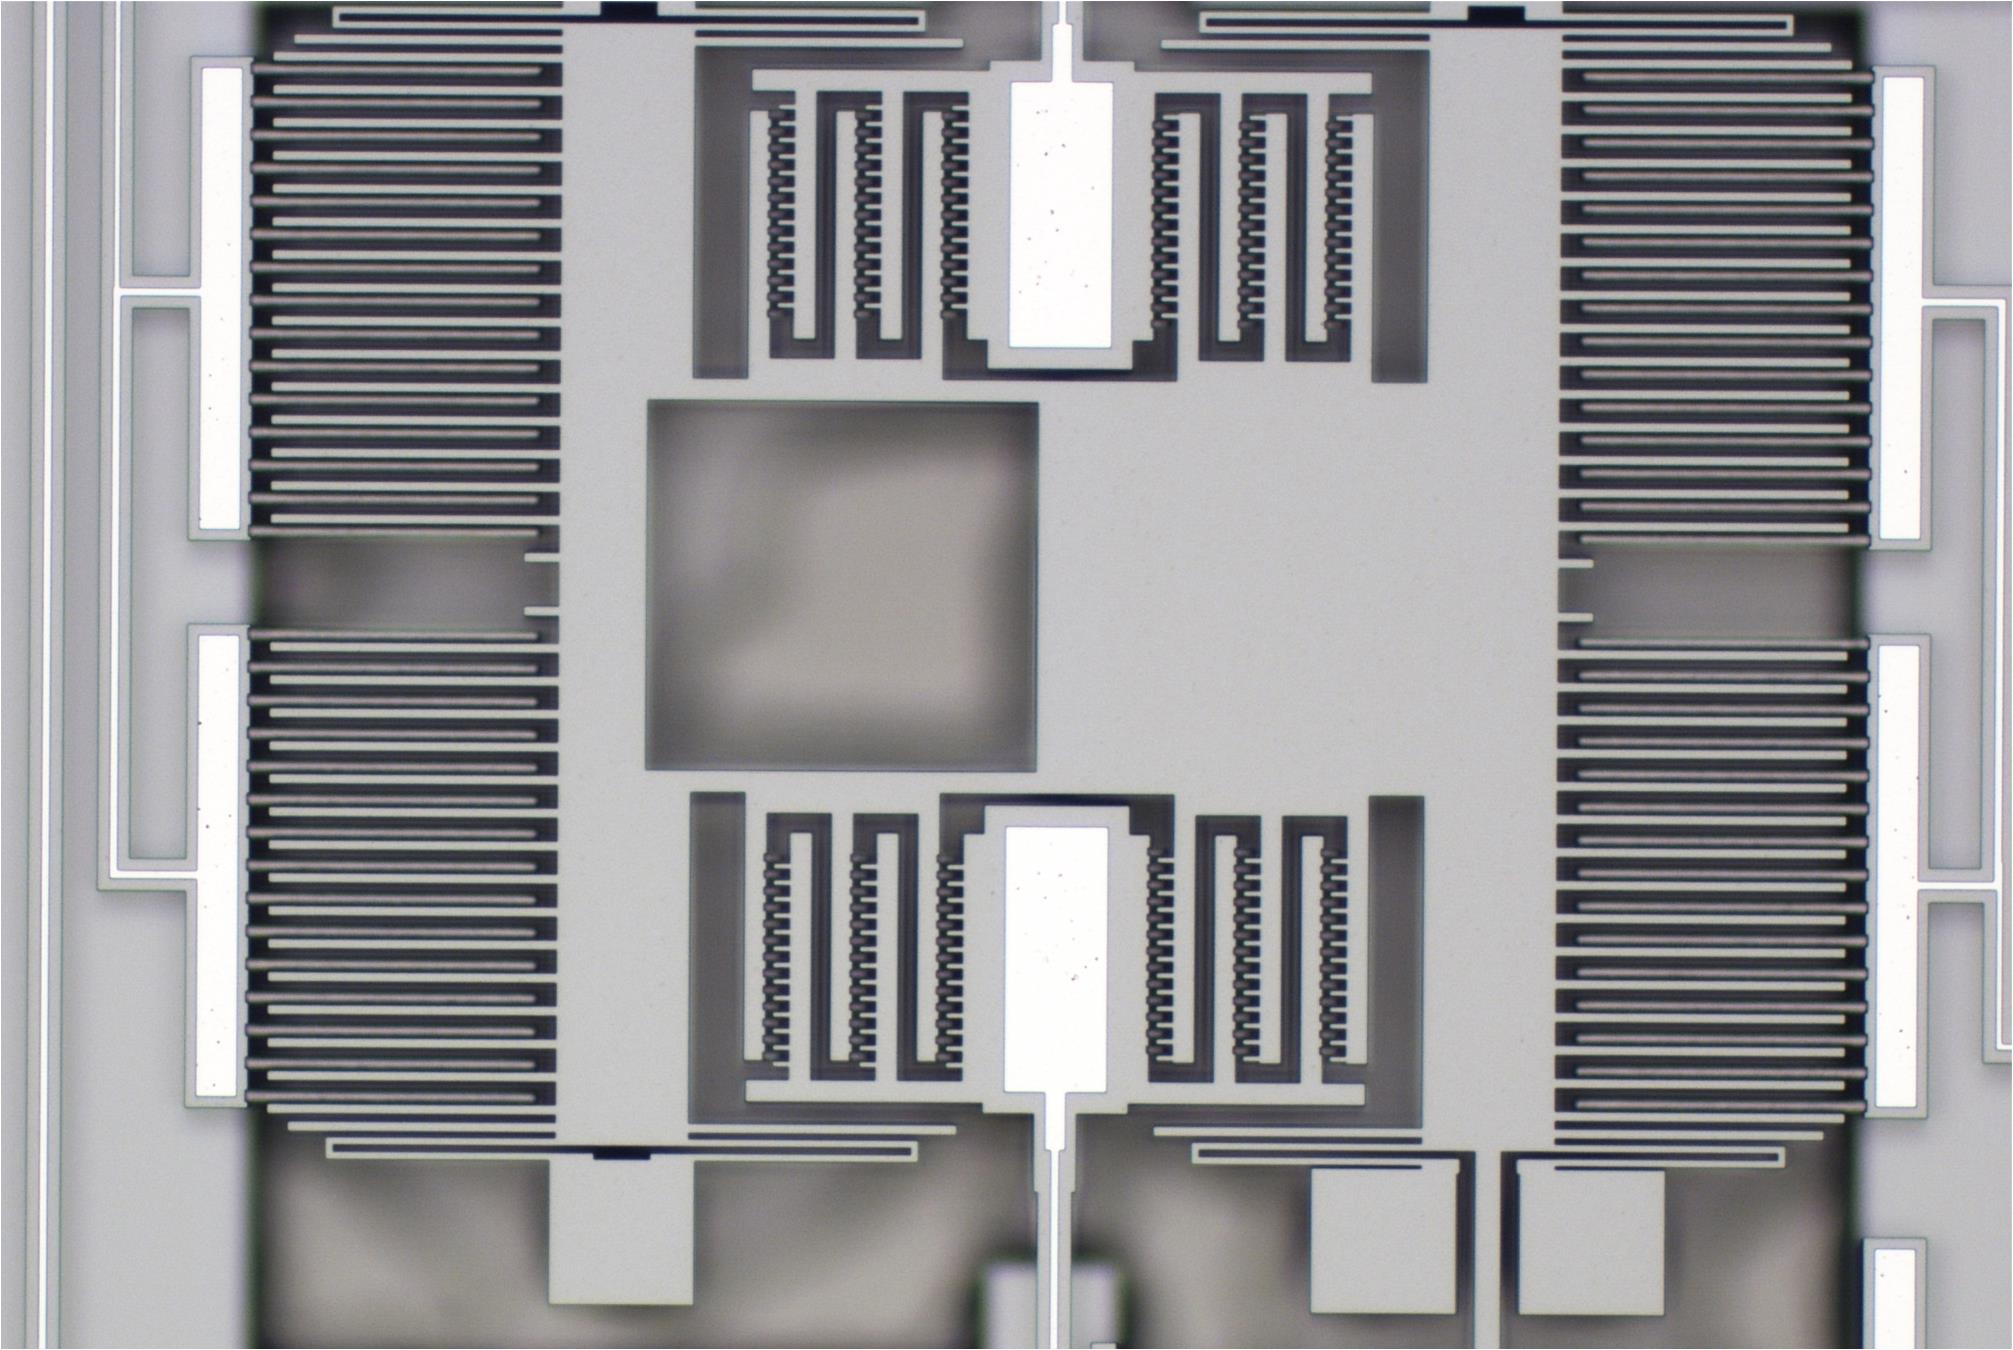
\includegraphics[height=3.2cm]{Figuras/acelerometro_mems_microscopia.png}}
	\hfill
	\subfloat[Esquema simplificado do acelerômetro capacitivo \cite{ufpr_accel}.]{%
		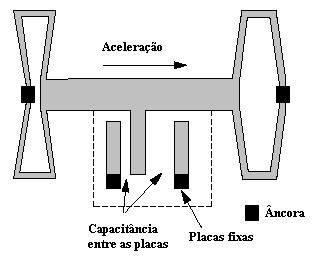
\includegraphics[height=3.2cm]{Figuras/acelerometro_esquema.png}}
	\caption{Estrutura interna de um acelerômetro MEMS capacitivo.}
	\label{fig:mems}
\end{figure}

\subsection{Tipos de Acelerômetros}
Existem diferentes tipos de acelerômetros, que se diferenciam pela forma como o deslocamento da massa é convertido em sinal elétrico. Nos piezoelétricos, a massa pressiona um cristal que gera carga elétrica proporcional à força, eles respondem bem a variações rápidas, mas não conseguem medir acelerações constantes, como a da gravidade \cite[pp.~187--189]{aguirre2013fundamentos}. Nos piezorresistivos, a deformação das molas altera a resistência de extensômetros ligados a elas. Já nos capacitivos, que é o caso do MPU 6050, o deslocamento altera a capacitância entre as placas, como descrito na seção anterior. Esse tipo consegue medir aceleração estática, como a da gravidade, o que é verificado na Seção~\ref{sec:verificacao}.

\subsection{Erros e Fontes de Incerteza}

Os erros nas medições de um acelerômetro MEMS podem decorrer de \textit{offset}, resolução limitada e desalinhamento em relação ao sistema de coordenadas de referência. Em movimentos de rotação, a distância entre o sensor e o centro de rotação também pode introduzir erros associados à aceleração angular. Esses fatores reduzem a precisão das medições e devem ser considerados na calibração \cite{Ghanipoor2020}.

\subsection{Acelerômetro do MPU 6050}
O MPU 6050 possui em um mesmo chip um acelerômetro e um giroscópio de três eixos. No acelerômetro, cada eixo possui a sua própria massa de prova, e o deslocamento dela é medido de forma diferencial por capacitores. Cada eixo tem um conversor analógico-digital sigma-delta de 16 bits e o fator de escala já vem calibrado de fábrica. Quando o sensor está parado sobre uma superfície plana, ele deve medir 0 g nos eixos X e Y e +1 g no eixo Z \cite{mpu6050}.

A comunicação com o sensor é feita pelo protocolo I$^2$C e a faixa de medição ($\pm 2$, $\pm 4$, $\pm 8$ ou $\pm 16$ g) é escolhida pelo registrador \texttt{ACCEL\_CONFIG}. Os valores lidos em cada eixo são convertidos para unidades de gravidade dividindo a leitura pela sensibilidade da faixa escolhida, que no caso de $\pm 2$~g é 16384~LSB/g.

\subsection{Característica do Sensor}

As características principais fornecidas pelo fabricante do sensor MPU 6050 são apresentadas na Tabela~\ref{tab:parametros}. A faixa de medição do sensor é de até $\pm 16\,\mathrm{g}$, com resolução a partir de $0{,}061\,\mathrm{mg/LSB}$ e sensibilidade de $16384\,\mathrm{LSB/g}$. Esses valores podem ser alterados entre 4 diferentes faixas de medição, configuradas a partir de um dos registradores do sensor. A não linearidade do sensor é de $0{,}5\%$ e o conversor analógico-digital tem resolução de 16 bits.

\begin{table}[!t]
	\caption{Parâmetros do sensor MPU 6050, extraídos do \textit{datasheet} \cite{mpu6050}.}
	\label{tab:parametros}
	\centering
	\renewcommand{\arraystretch}{1.3}
	\setlength{\tabcolsep}{5pt}
	\begin{tabular}{|l|c|c|c|c|} \hline
		\textbf{Parâmetro} & \textbf{Mín.} & \textbf{Típ.} & \textbf{Máx.} & \textbf{Unid.} \\ \hline
		Resolução do ADC & & 16 & & bits \\ \hline
		Faixa nominal & $\pm 2$ & & $\pm 16$ & g \\ \hline
		Sensibilidade & 2048 & & 16384 & LSB/g \\ \hline
		Resolução & 0,061 & & 0,488 & mg/LSB \\ \hline
		Não linearidade & & 0,5 & & \% \\ \hline
		\textit{Offset} zero-g (X e Y) & & $\pm 50$ & & mg \\ \hline
		\textit{Offset} zero-g (Z) & & $\pm 80$ & & mg \\ \hline
		Sensibilidade cruzada & & $\pm 2$ & & \% \\ \hline
		Densidade de ruído & & 400 & & $\mu$g/$\sqrt{\mathrm{Hz}}$ \rule[-1.2ex]{0pt}{3.6ex} \\ \hline
	\end{tabular}
\end{table}

\section{Verificação Experimental}
\label{sec:verificacao}
A Figura~\ref{fig:montagem} mostra a montagem utilizada, com o MPU 6050 ligado a um ESP32 pelo barramento I$^2$C, e a Figura~\ref{fig:esquematico} mostra o esquemático das ligações.

\begin{figure}[!t]
	\centering
	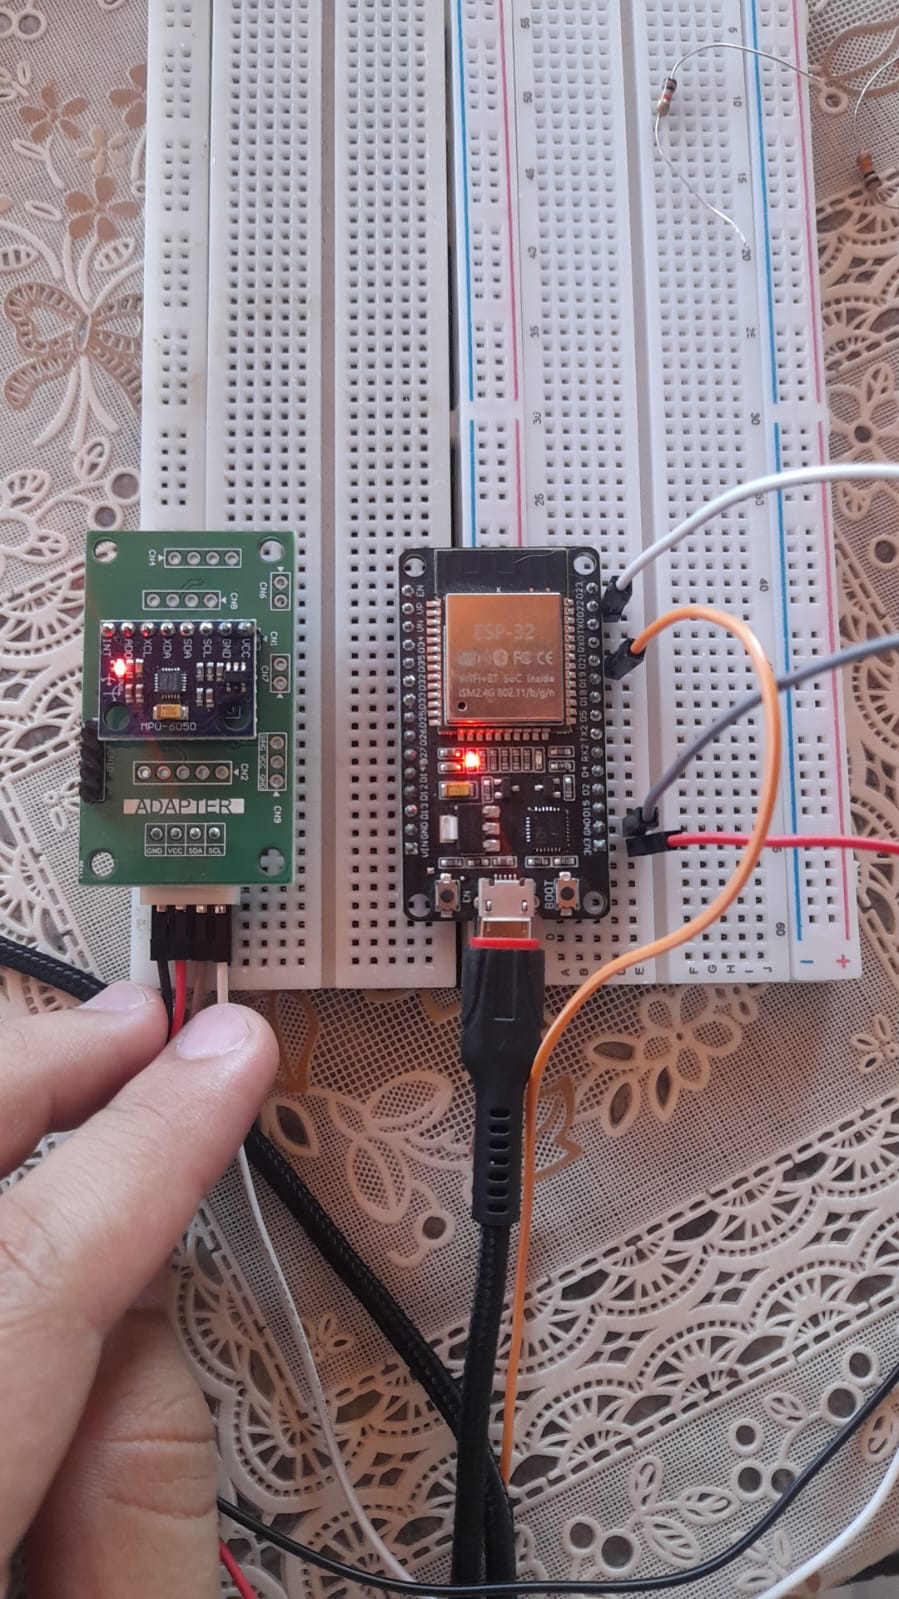
\includegraphics[width=0.8\columnwidth, trim=50bp 600bp 19bp 470bp, clip]{Figuras/montagem_esp32_mpu6050.png}
	\caption{Montagem utilizada: MPU 6050 (à esquerda) ligado ao ESP32 (à direita).}
	\label{fig:montagem}
\end{figure}

\begin{figure}[!t]
	\centering
	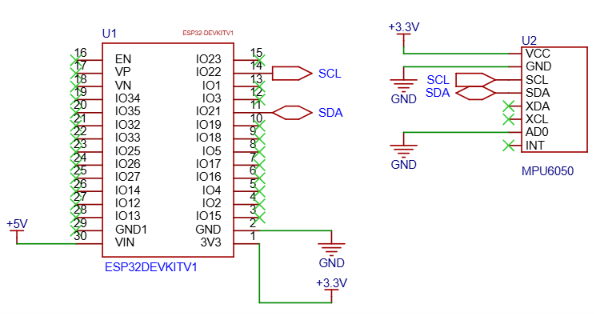
\includegraphics[width=\columnwidth]{Figuras/esquematico.png}
	\caption{Esquemático das ligações entre o ESP32 e o MPU 6050.}
	\label{fig:esquematico}
\end{figure}

O sensor foi mantido em repouso sobre a bancada em seis posições, duas para cada eixo, girando a placa para que a gravidade apontasse primeiro no sentido positivo e depois no sentido negativo do eixo em teste. Em cada posição foram registrados cerca de 10 segundos de leitura simultânea dos três eixos. A Figura~\ref{fig:verificacao_experimental} reúne os seis ensaios.

Em todos eles o eixo alinhado com a vertical fica próximo de $\pm 1\,\mathrm{g}$ e os outros dois, perto de zero, como se espera do sensor em repouso. As leituras não coincidem exatamente com esses valores: o eixo Z, por exemplo, indica cerca de $0{,}1\,\mathrm{g}$ nos ensaios em que deveria ler zero. Esse desvio soma o erro de zero do próprio sensor, informado no \textit{datasheet}, ao desalinhamento entre a placa e a horizontal, já que a superfície de apoio não está perfeitamente nivelada.

\begin{figure*}[!t]
	\centering
	\subfloat[Placa apoiada na borda, com o eixo X na vertical. X fica em torno de $+1\,g$.\label{fig:x_positivo}]{%
		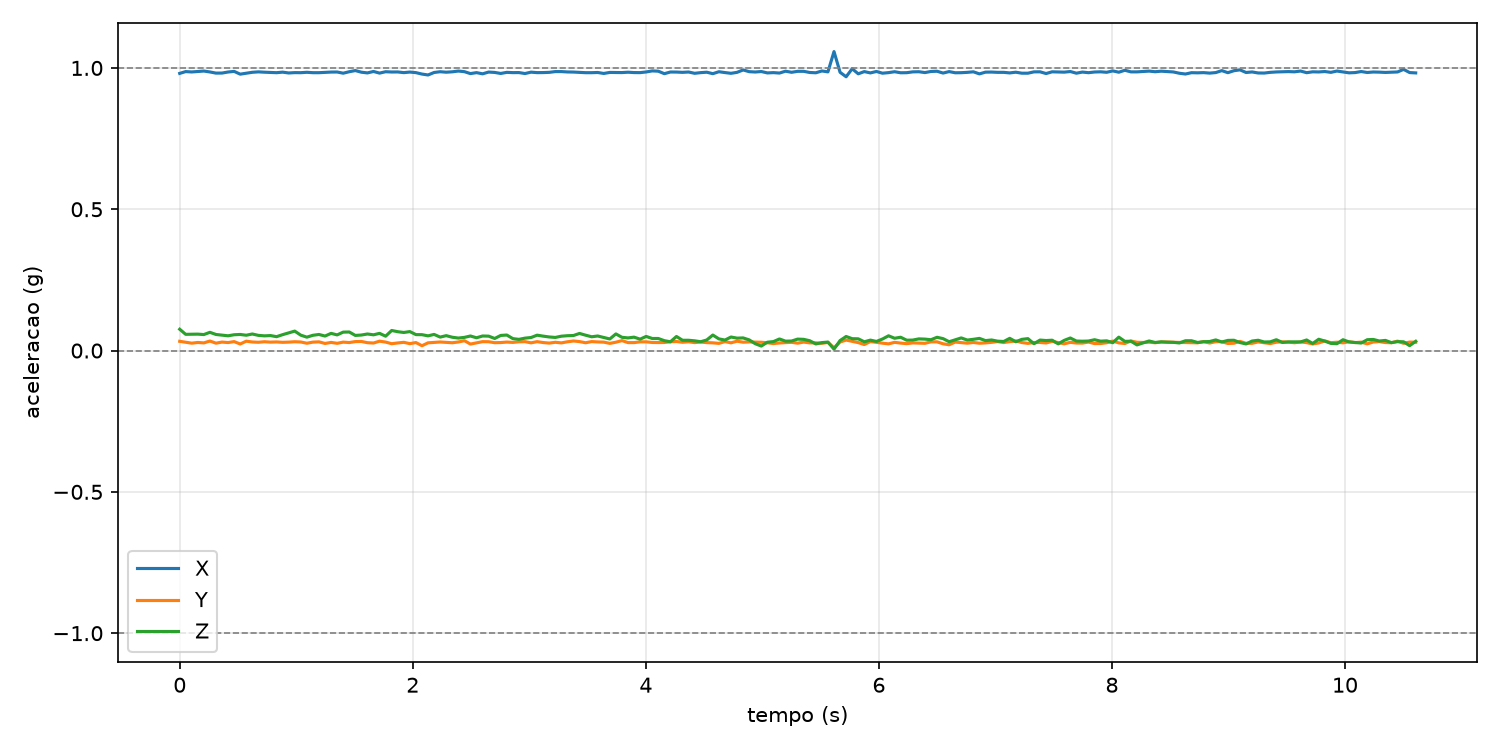
\includegraphics[width=0.47\textwidth]{Figuras/apoiado_na_borda_X_para_baixo.png}}
	\hfill
	\subfloat[A mesma placa virada para a borda oposta. O eixo X passa a marcar cerca de $-1\,g$.\label{fig:x_negativo}]{%
		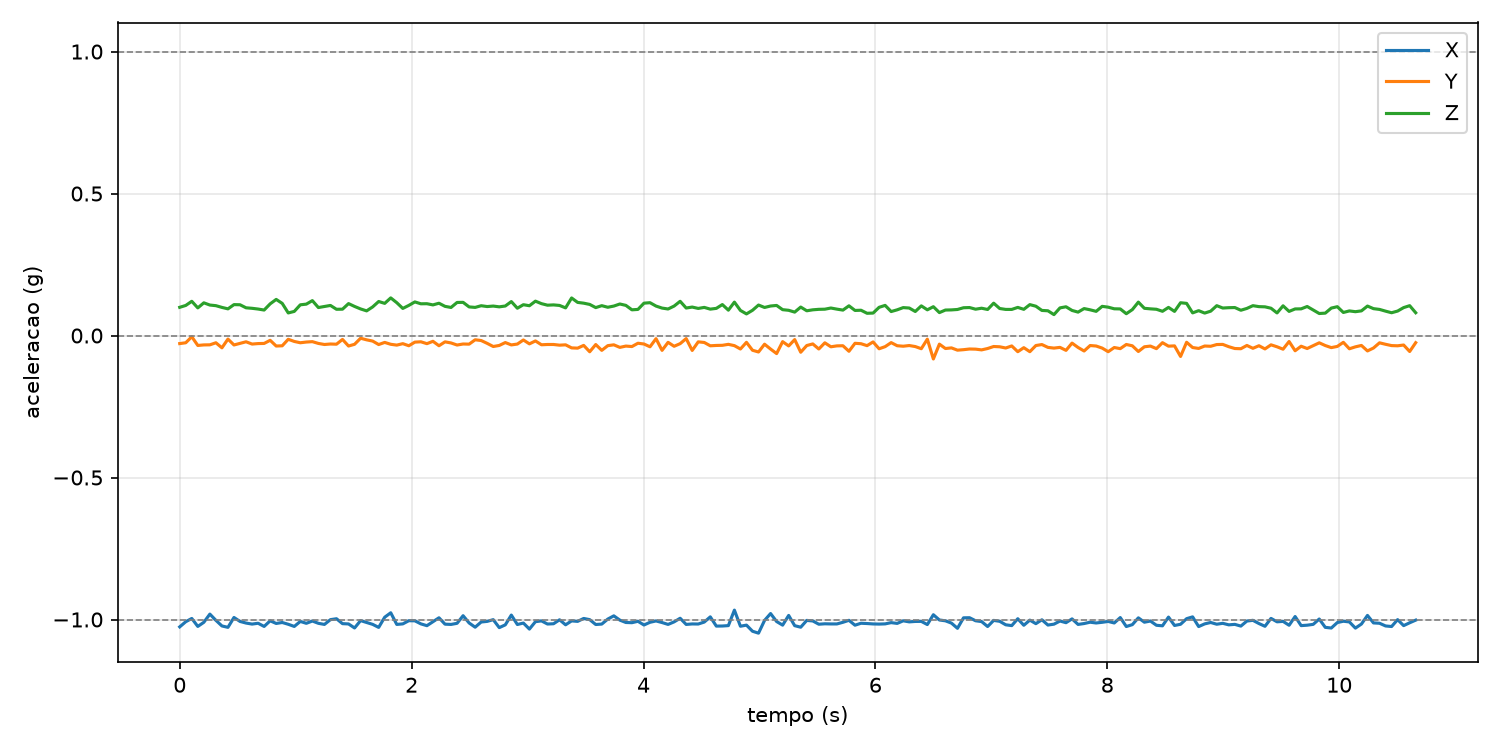
\includegraphics[width=0.47\textwidth]{Figuras/borda_oposta_X_para_cima.png}}

	\subfloat[Placa apoiada na borda com o eixo Y na vertical, lendo perto de $+1\,g$.\label{fig:y_positivo}]{%
		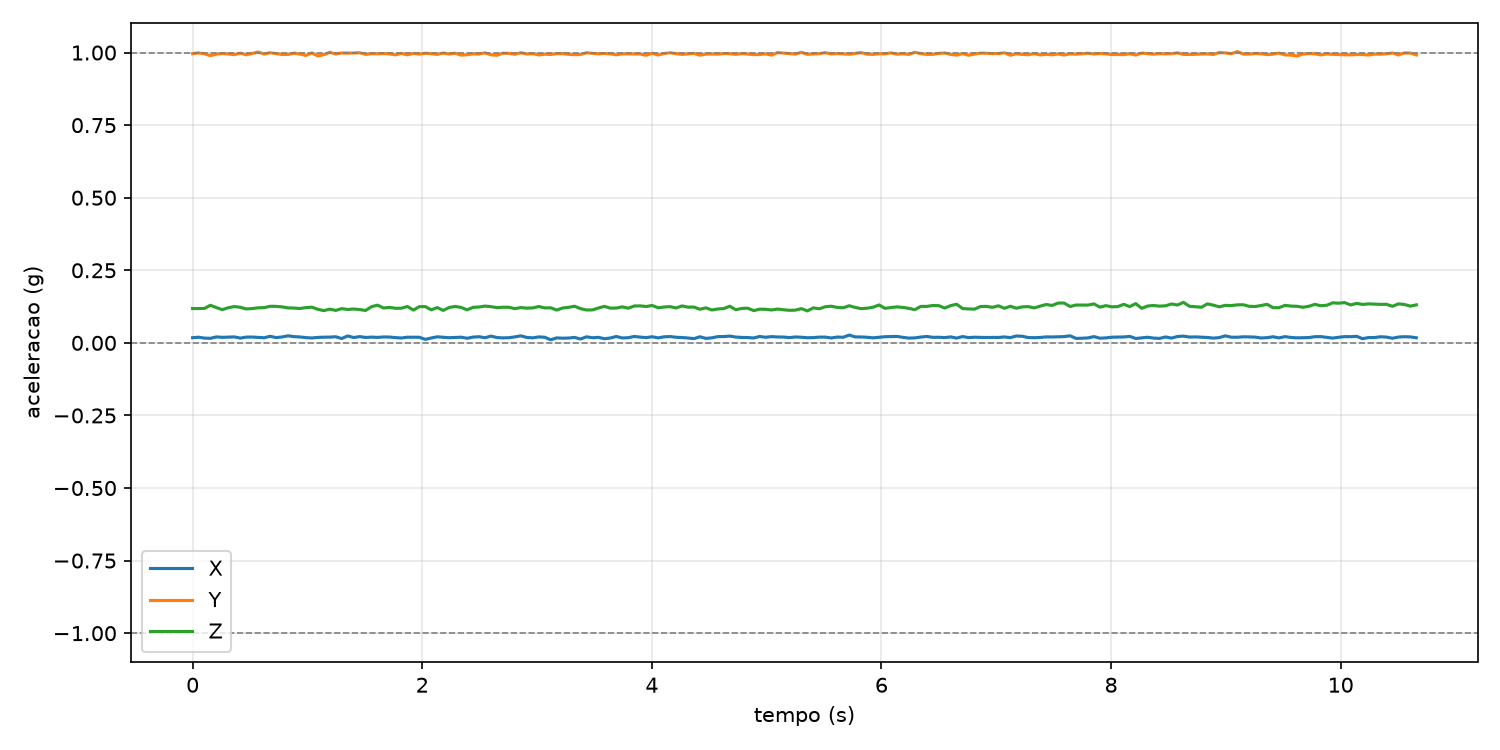
\includegraphics[width=0.47\textwidth]{Figuras/apoiado_na_borda_Y_para_baixo.png}}
	\hfill
	\subfloat[Borda oposta, eixo Y invertido: a leitura cai para cerca de $-1\,g$.\label{fig:y_negativo}]{%
		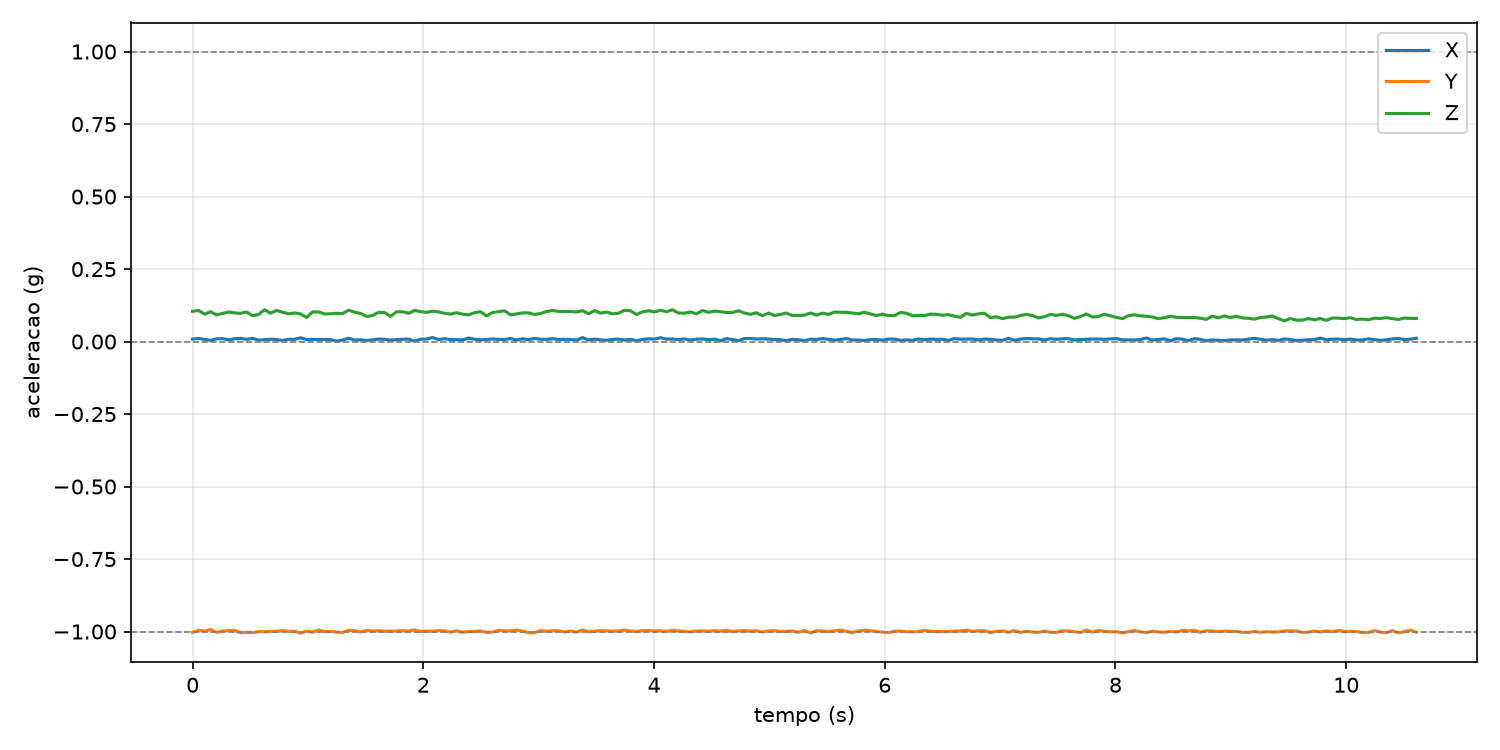
\includegraphics[width=0.47\textwidth]{Figuras/borda_oposta_Y_para_cima.png}}

	\subfloat[Placa deitada, componentes voltados para cima. Z marca pouco mais de $+1\,g$.\label{fig:z_positivo}]{%
		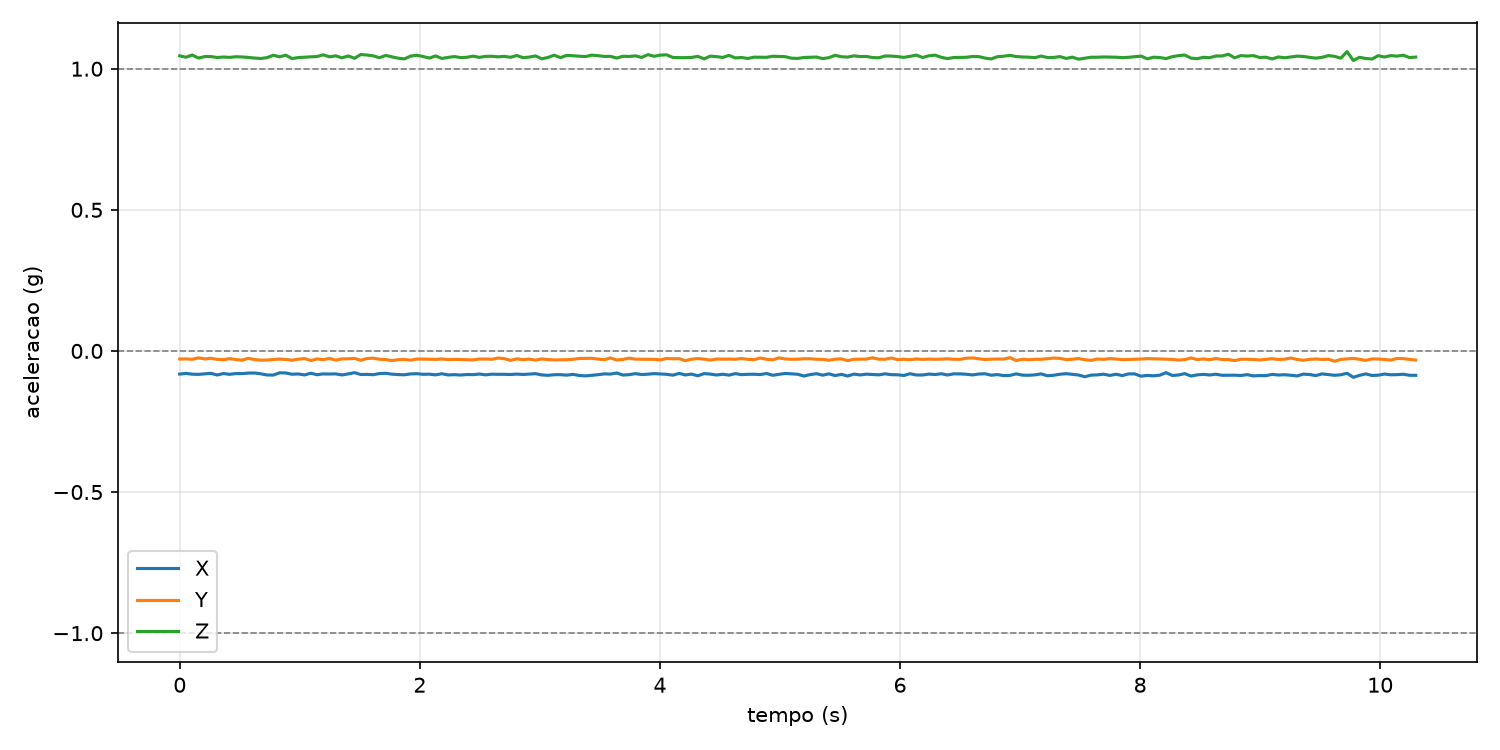
\includegraphics[width=0.47\textwidth]{Figuras/deitado_componentes_para_cima_Z.png}}
	\hfill
	\subfloat[Placa deitada de cabeça para baixo, com Z em torno de $-1\,g$.\label{fig:z_negativo}]{%
		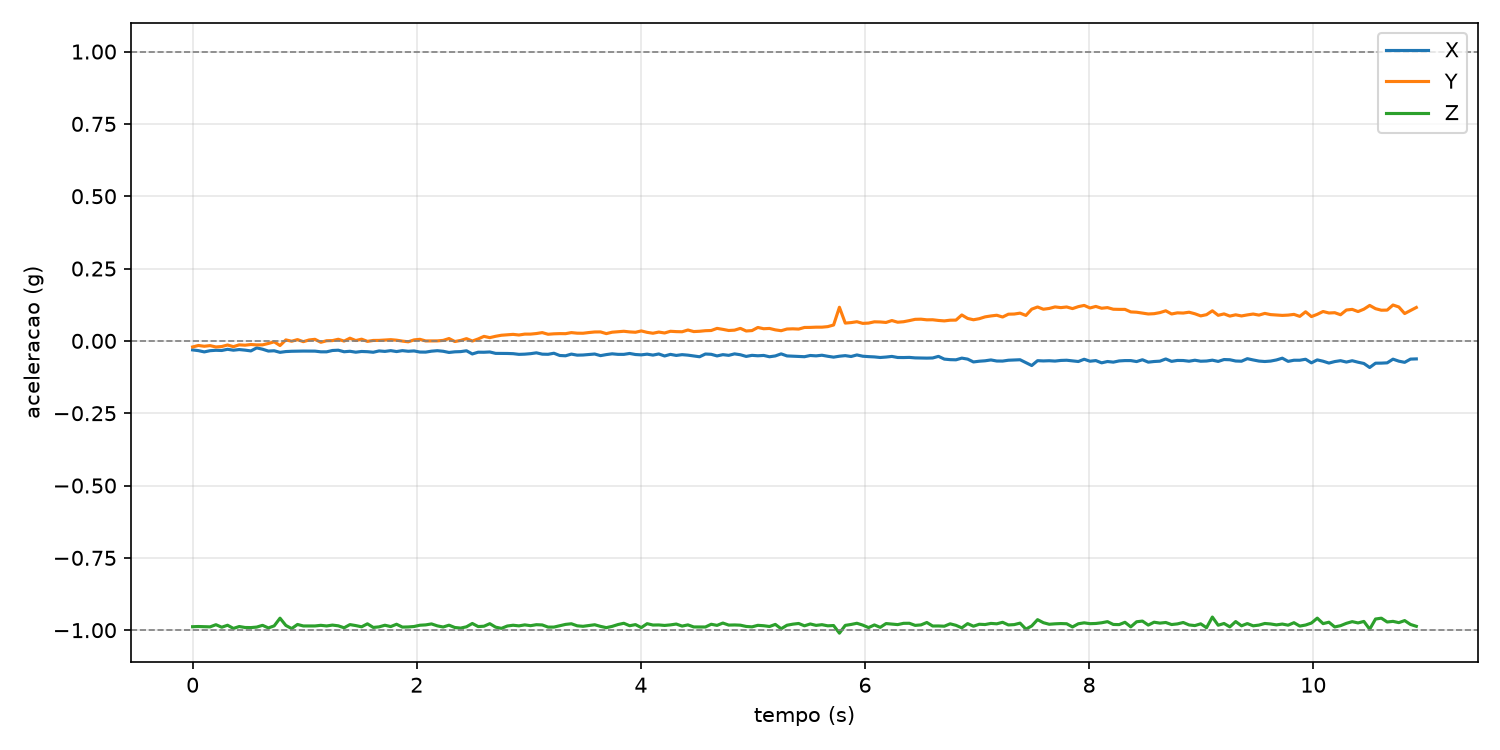
\includegraphics[width=0.47\textwidth]{Figuras/deitado_de_cabeca_para_baixo_Z.png}}
	\caption{Aceleração medida nos três eixos do MPU 6050 com o sensor parado, nas seis posições de ensaio, na ordem dos eixos X, Y e Z.}
	\label{fig:verificacao_experimental}
\end{figure*}

% ---------------------------------------------------------------------------
% Seções da Entrega 2 (ver entrega2_02_2026.pdf). Escrever aqui.
% ---------------------------------------------------------------------------

\section{Desenvolvimento}

\subsection{Calibração Estática}
A saída de cada eixo do acelerômetro foi representada pela relação linear proposta no roteiro,
\begin{equation}
	A_{\text{saída}} = \text{Ganho} \times A_{\text{ref}} + A_{\text{offset}},
	\label{eq:modelo}
\end{equation}
em que $A_{\text{saída}}$ é o valor lido em g, $A_{\text{ref}}$ é a aceleração de referência, que neste caso é $\pm1$\,g, o ganho é adimensional e $A_{\text{offset}}$ é um erro fixo, em g, que se soma a todas as leituras do eixo.

Para a calibração, o sensor foi apoiado sobre uma superfície nivelada com o auxílio de um nível de bolha, em seis posições: para cada eixo, uma com o eixo apontando para cima ($+1$\,g) e outra com o eixo apontando para baixo ($-1$\,g). O sensor foi configurado na faixa de $\pm2$\,g, a de maior sensibilidade (16384~LSB/g), já que parado ele só mede a gravidade. Em cada posição foram gravadas 200 leituras, o dobro do mínimo pedido, com uma leitura a cada 52~ms, o que dá cerca de 10~s por posição.

Com as médias $\bar{A}_{+1g,i}$ e $\bar{A}_{-1g,i}$ de cada eixo $i$, a Equação~\eqref{eq:modelo} gera um sistema de duas equações:
\begin{align}
	\bar{A}_{+1g,i} &= \text{Ganho}_i \times (1\,\text{g}) + A_{\text{offset},i} \label{eq:sis1}\\
	\bar{A}_{-1g,i} &= \text{Ganho}_i \times (-1\,\text{g}) + A_{\text{offset},i} \label{eq:sis2}
\end{align}
Subtraindo uma equação da outra o offset é eliminado, e somando as duas o ganho é eliminado:
\begin{equation}
	\text{Ganho}_i = \frac{\bar{A}_{+1g,i} - \bar{A}_{-1g,i}}{2}, \quad
	A_{\text{offset},i} = \frac{\bar{A}_{+1g,i} + \bar{A}_{-1g,i}}{2}.
	\label{eq:solucao}
\end{equation}

Os valores obtidos estão na Tabela~\ref{tab:calibracao}. Os ganhos ficaram entre 0,9988 e 1,0153. Os offsets dos eixos X e Y ficaram abaixo de 3~mg, e o do eixo Z foi de 34,4~mg, dentro do valor típico de $\pm80$~mg informado no \textit{datasheet} (Tabela~\ref{tab:parametros}). Esses valores foram gravados no firmware, que corrige cada leitura antes de calcular o ângulo:
\begin{equation}
	A_{\text{corrigida}} = \frac{A_{\text{saída}} - A_{\text{offset}}}{\text{Ganho}}.
	\label{eq:correcao}
\end{equation}

\begin{table}[!htb]
	\caption{Ganho e \textit{offset} estimados para cada eixo.}
	\label{tab:calibracao}
	\centering
	\renewcommand{\arraystretch}{1.3}
	\begin{tabular}{|c|c|c|c|c|} \hline
		\textbf{Eixo} & $\bar{A}_{+1g}$ (g) & $\bar{A}_{-1g}$ (g) & \textbf{Ganho} & \textbf{\textit{Offset}} (g) \\ \hline
		X & 0{,}9960 & $-1{,}0015$ & 0{,}9988 & $-0{,}0028$ \\ \hline
		Y & 1{,}0012 & $-0{,}9997$ & 1{,}0004 & 0{,}0007 \\ \hline
		Z & 1{,}0497 & $-0{,}9810$ & 1{,}0153 & 0{,}0344 \\ \hline
	\end{tabular}
\end{table}

\subsection{Cálculo do Ângulo de Inclinação}
O módulo foi fixado no mecanismo com o eixo X do sensor alinhado ao eixo de giro. Dessa forma, com o braço parado, a gravidade fica sempre no plano formado pelos eixos Y e Z do sensor e o eixo X lê perto de zero; nos ensaios, a média de X ficou entre $-0{,}018$ e $0{,}022$\,g. Com o braço em $0^\circ$ o eixo Y aponta para cima e mede 1\,g. Ao girar o braço de um ângulo $\theta$, as leituras corrigidas de Y e Z passam a ser as projeções da gravidade nesses eixos,
\begin{equation}
	c_y = \cos\theta, \qquad c_z = \sin\theta,
	\label{eq:projecoes}
\end{equation}
e o ângulo é calculado por
\begin{equation}
	\theta = \operatorname{atan2}(c_z,\, c_y).
	\label{eq:atan2}
\end{equation}

Esse cálculo da inclinação a partir de dois eixos é descrito nas notas de aplicação da Freescale \cite{pedley2013} e da Analog Devices \cite{fisher2010}. A função atan2 usa o sinal das duas componentes e devolve o ângulo entre $-180^\circ$ e $180^\circ$, sem a divisão por zero que aparece em $\arctan(c_z/c_y)$ quando $\theta = 90^\circ$. Usar os dois eixos também evita a perda de sensibilidade que o cálculo com um eixo só, $\theta = \arcsin(c_z)$, tem perto de $90^\circ$ \cite{fisher2010}. Como o resultado do atan2 passa de $+180^\circ$ para $-180^\circ$ no fim da faixa do transferidor, o programa soma $360^\circ$ quando o ângulo fica abaixo de $-90^\circ$, e assim a faixa de $0^\circ$ a $180^\circ$ fica contínua.

A Figura~\ref{fig:pseudocodigo} mostra o pseudocódigo do programa do ESP32. A cada 50~ms ele lê os três eixos, aplica a correção da Equação~\eqref{eq:correcao}, calcula o ângulo e envia os dados pela serial. No computador, um script em Python grava os dados em arquivos CSV e outro calcula o ganho e o offset a partir das seis posições. Todos os códigos estão no repositório do grupo\footnote{\url{https://github.com/Gabreeles/instrumentacao_eletronica_2026_2}}.

\begin{figure}[!t]
	\begin{algorithmic}[1]
		\STATE configurar o MPU 6050 na faixa de $\pm 2$~g
		\LOOP
		\STATE ler $a_x$, $a_y$, $a_z$ e dividir por 16384~LSB/g
		\STATE corrigir cada eixo: $c_i \leftarrow (a_i - \text{Offset}_i)/\text{Ganho}_i$
		\STATE $\theta \leftarrow \operatorname{atan2}(c_z, c_y) \cdot 180/\pi$
		\IF{$\theta < -90^\circ$}
		\STATE $\theta \leftarrow \theta + 360^\circ$
		\ENDIF
		\STATE enviar $t$, $a_x$, $a_y$, $a_z$ e $\theta$ pela serial
		\STATE esperar 50~ms
		\ENDLOOP
	\end{algorithmic}
	\caption{Pseudocódigo do programa do ESP32.}
	\label{fig:pseudocodigo}
\end{figure}

\subsection{Mecanismo de Validação}
Para a validação foi projetada e impressa em 3D a base das Figuras~\ref{fig:base} e~\ref{fig:base_real}. O módulo é parafusado em um berço, que gira em torno de um eixo horizontal apoiado em um quadro, e por isso o conjunto tem um grau de liberdade, como o braço mecânico sugerido no roteiro. Um dos eixos laterais tem um pino mais curto que, apertado contra o quadro, trava o berço na posição desejada, e os dois eixos têm marcas a cada $15^\circ$. A base também tem uma escala de giro horizontal, que não foi usada neste trabalho.
% TODO: dizer como o transferidor foi acoplado e qual a menor divisão dele.

\begin{figure}[!t]
	\centering
	\subfloat[Vista frontal.]{%
		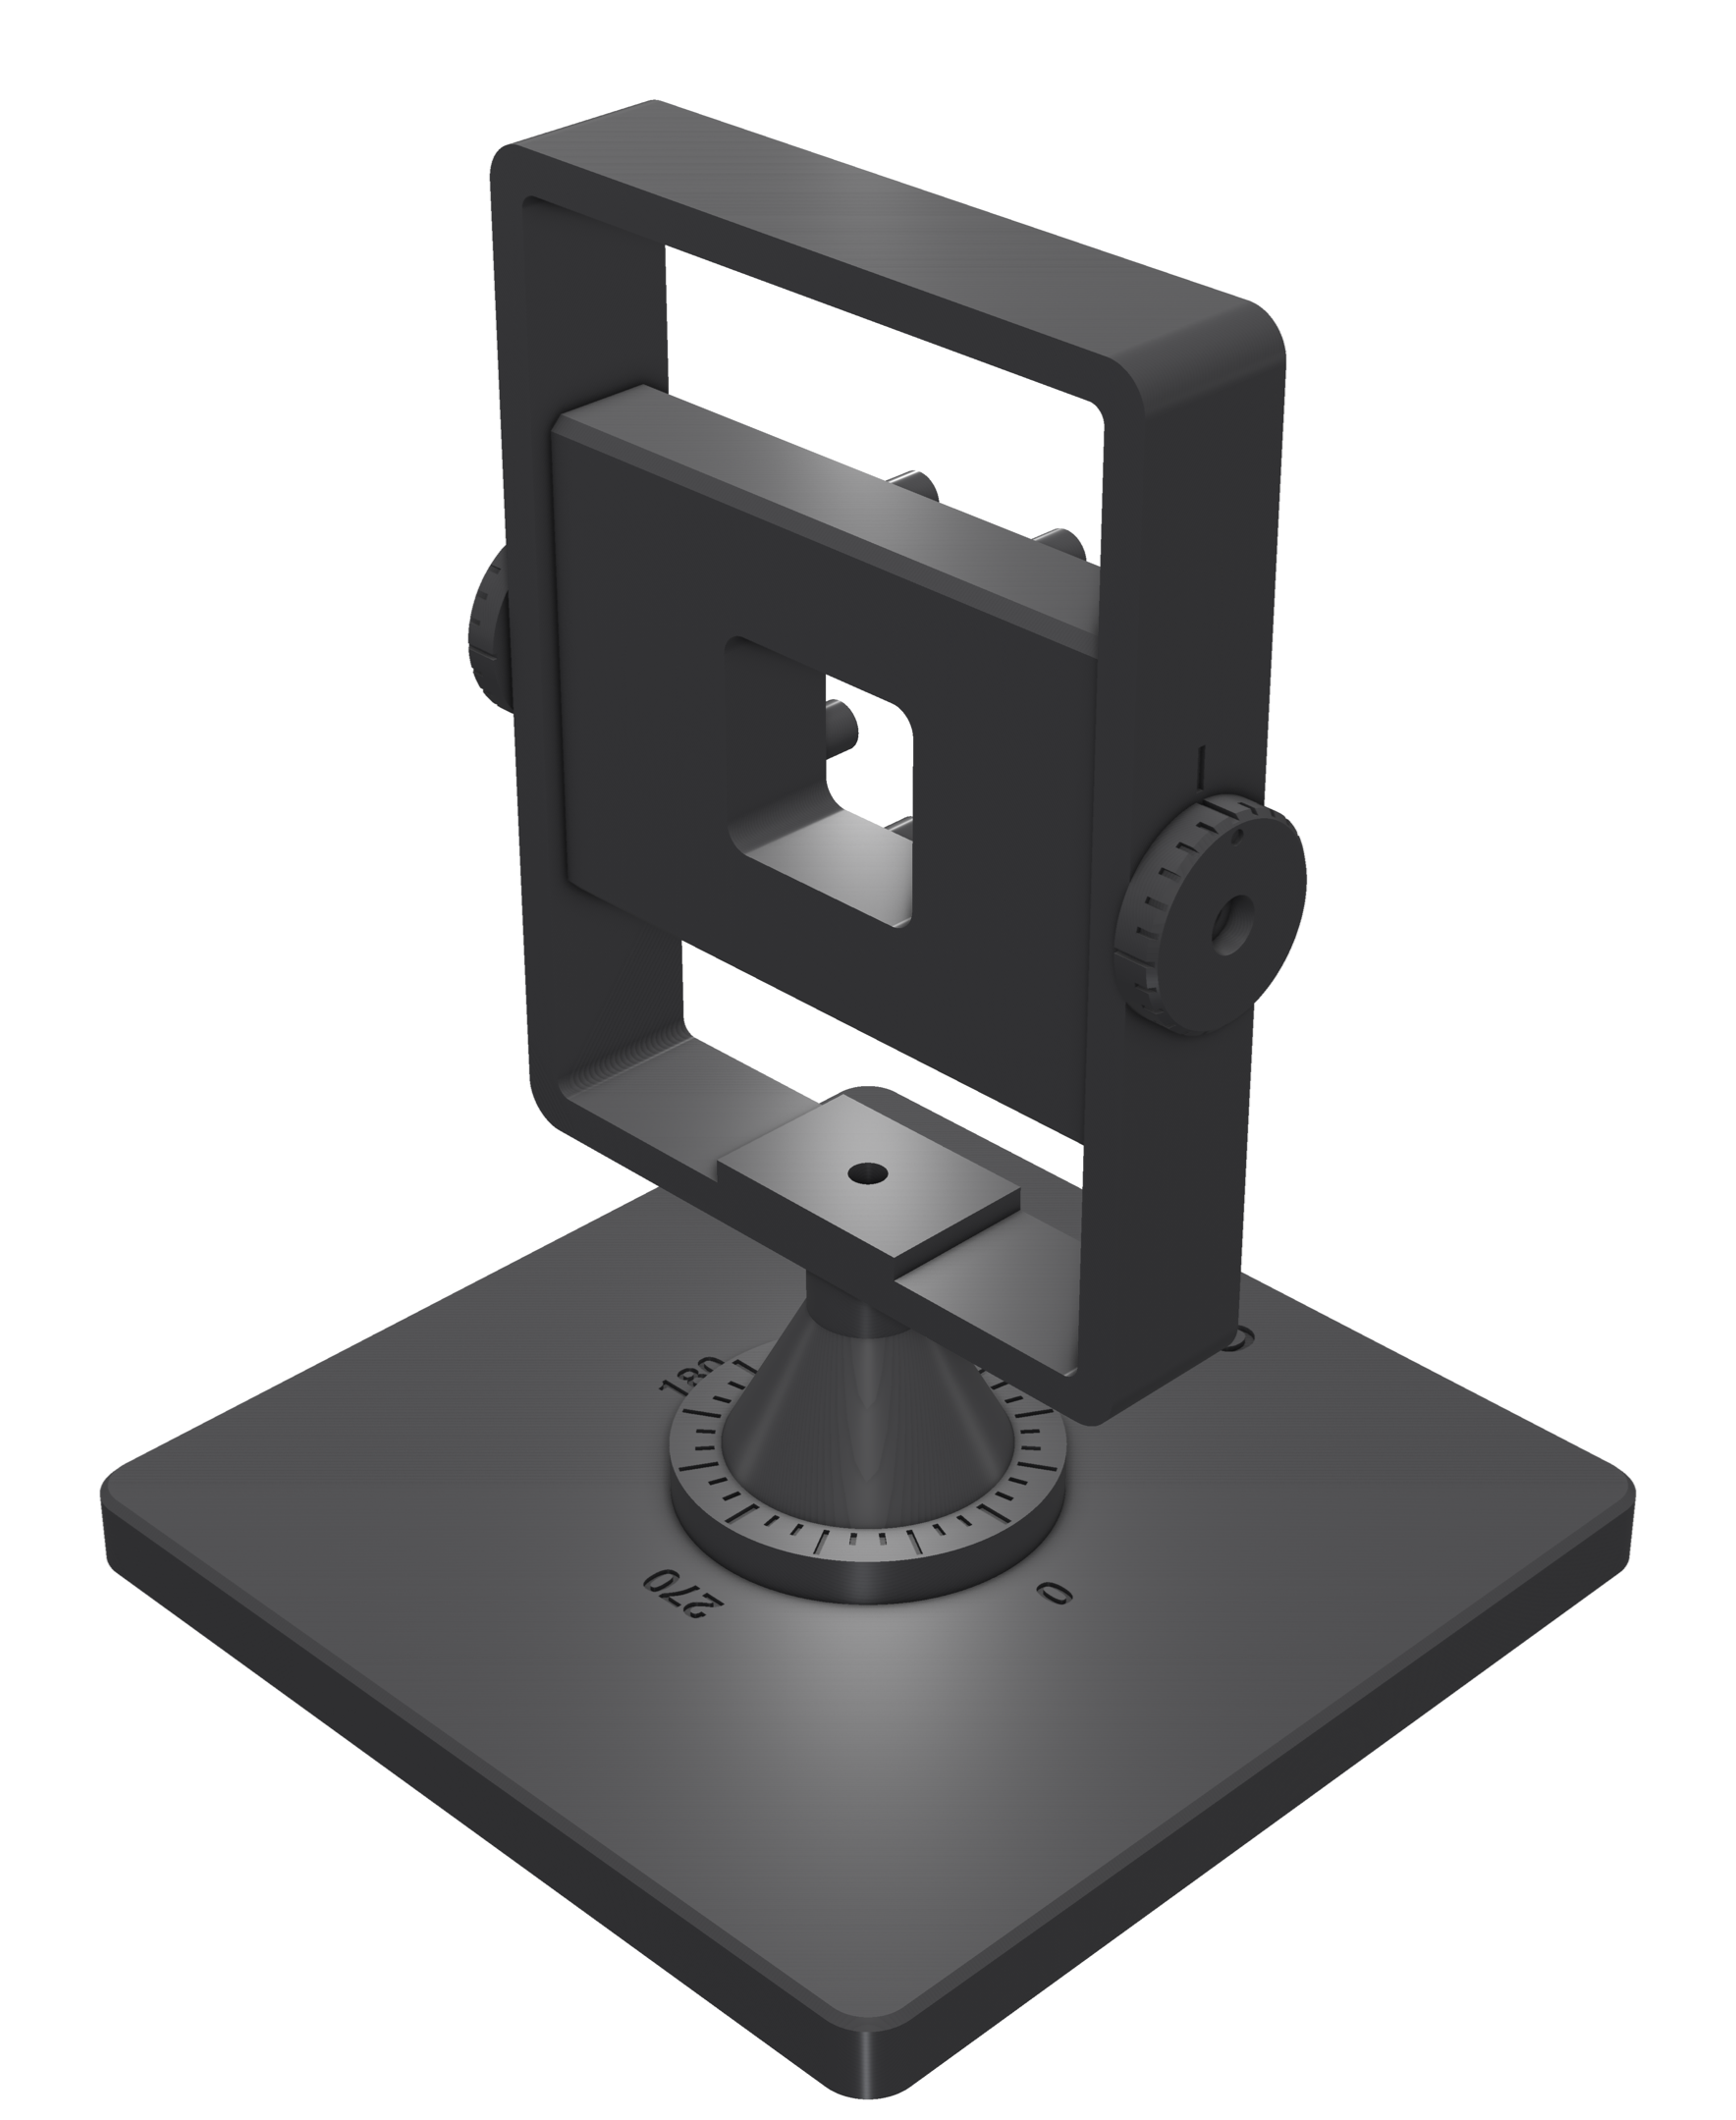
\includegraphics[width=0.48\columnwidth]{Figuras/montagem_render_frente.png}}
	\hfill
	\subfloat[Vista traseira.]{%
		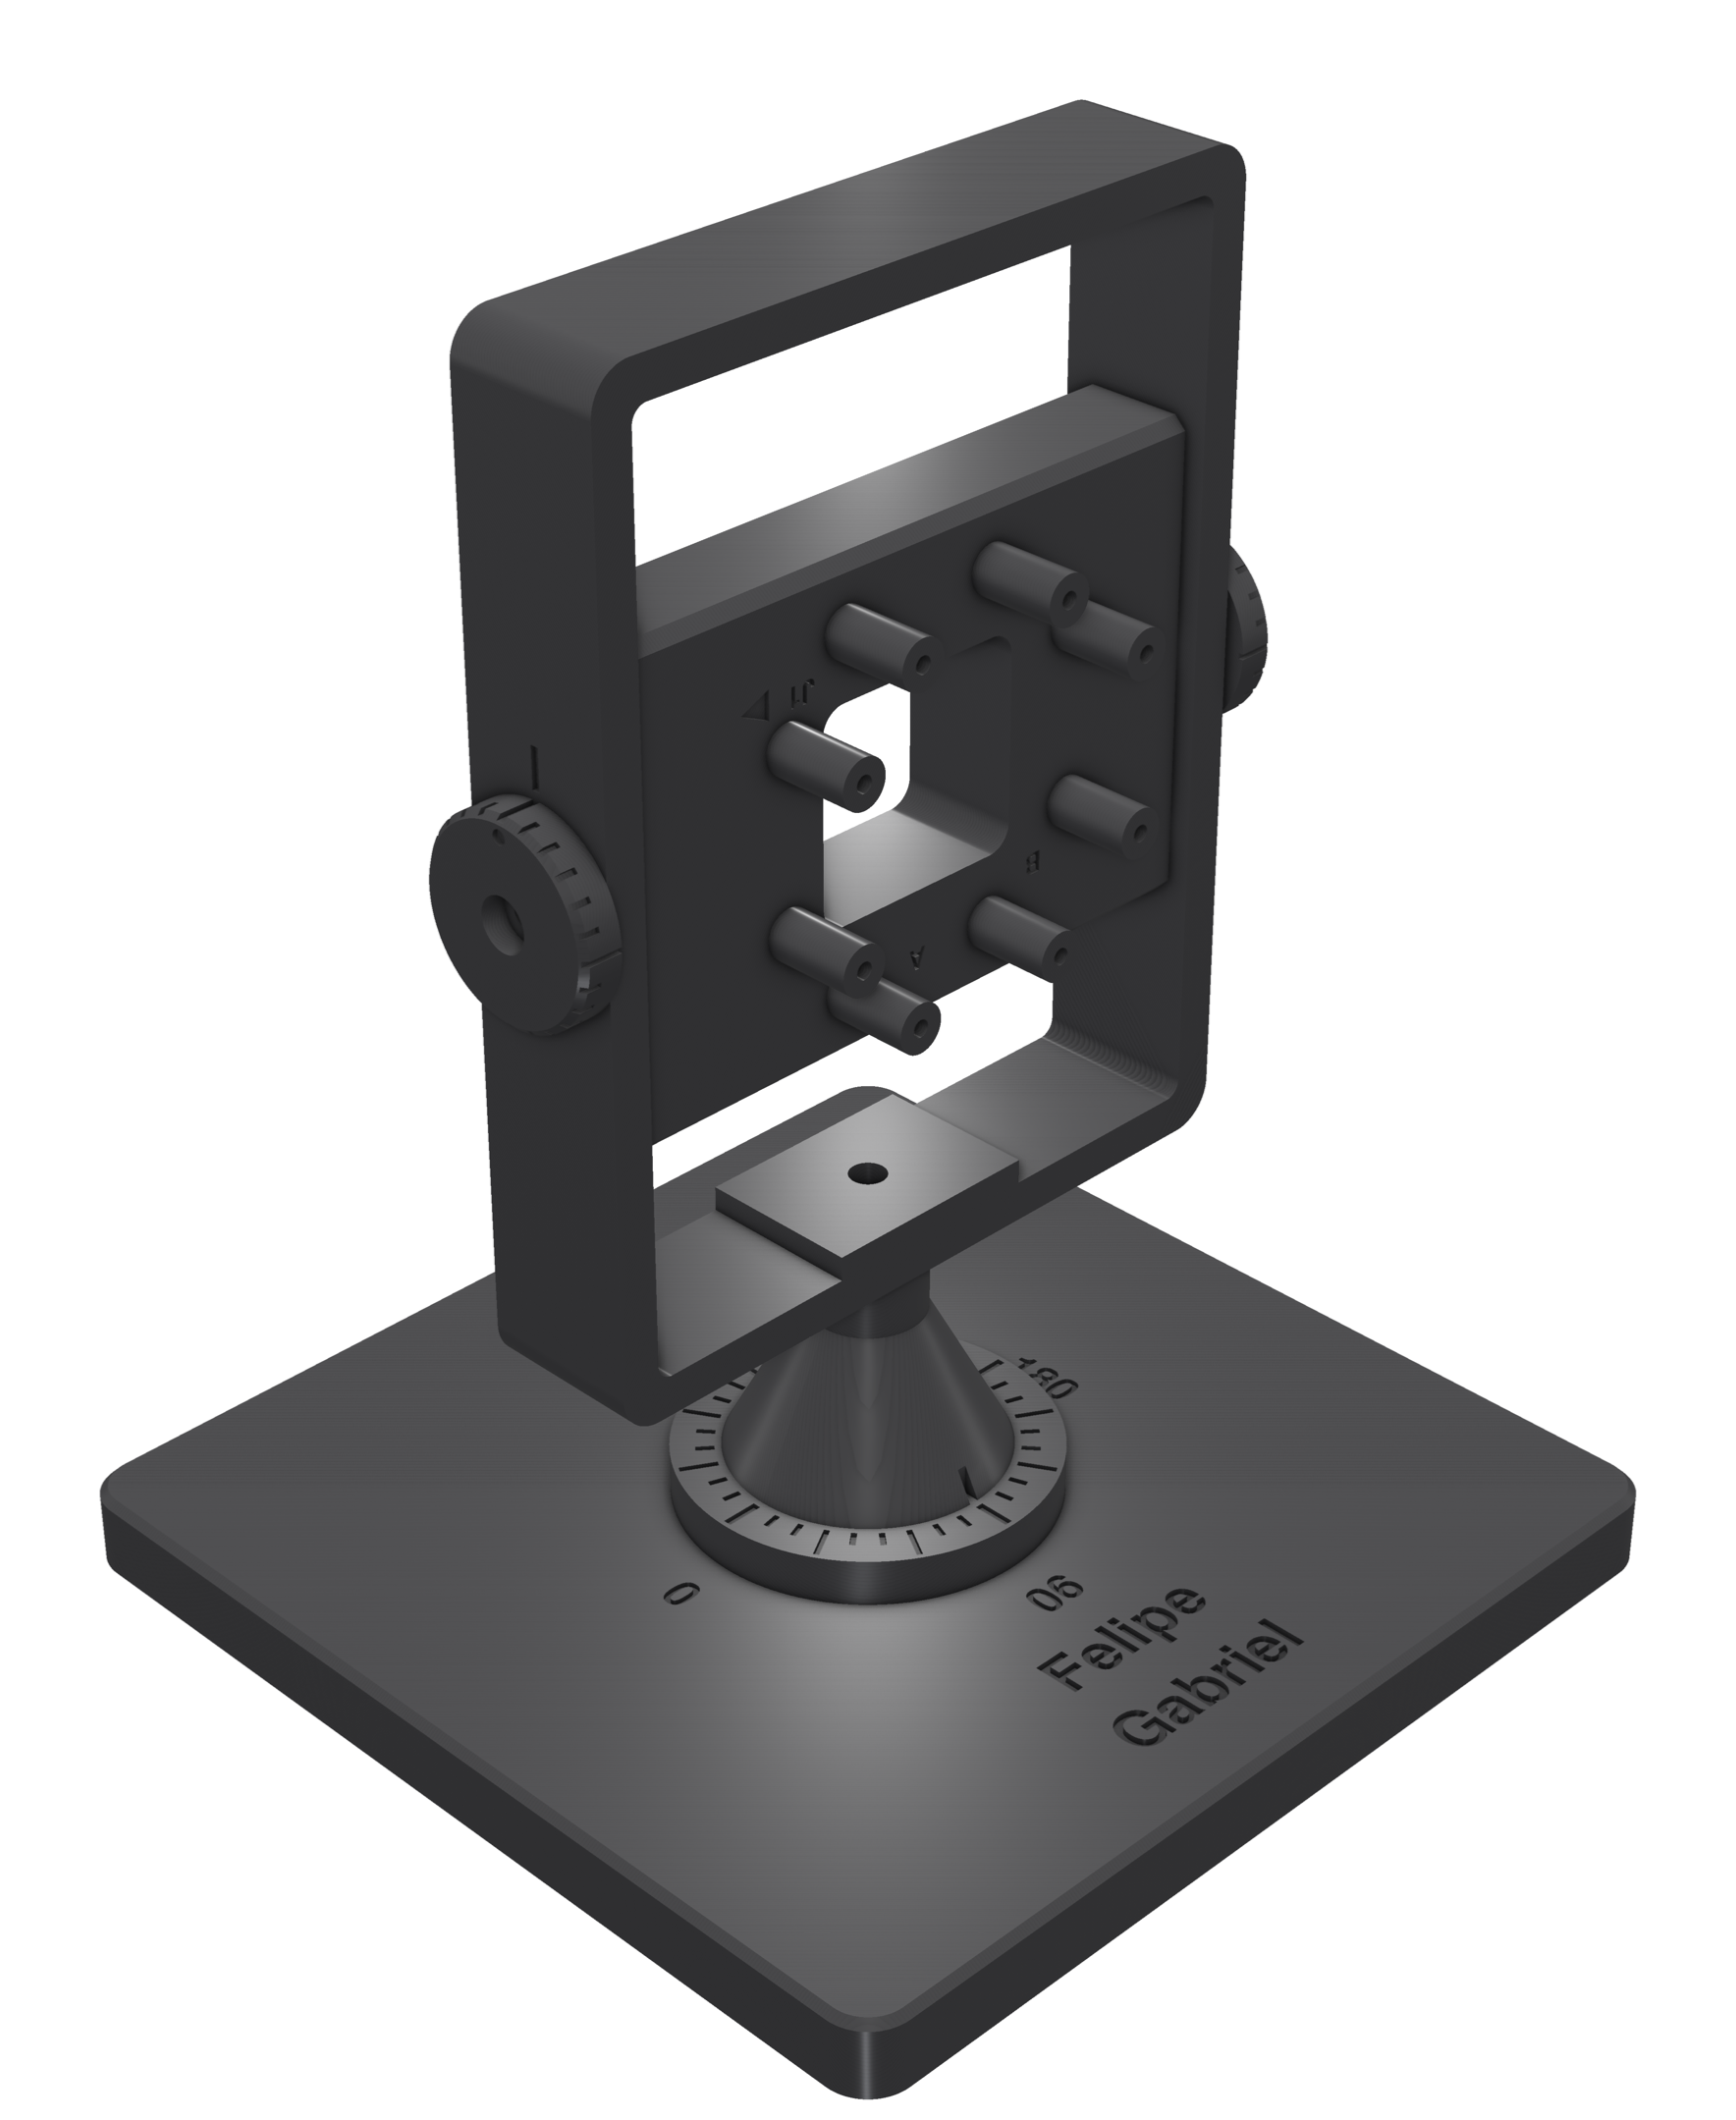
\includegraphics[width=0.48\columnwidth]{Figuras/montagem_render_verso.png}}
	\caption{Modelo 3D da base do MPU 6050, com escala de giro horizontal na base e eixos de giro com escala a cada $15^\circ$.}
	\label{fig:base}
\end{figure}

\begin{figure}[!t]
	\centering
	\subfloat[Vista isométrica.]{
		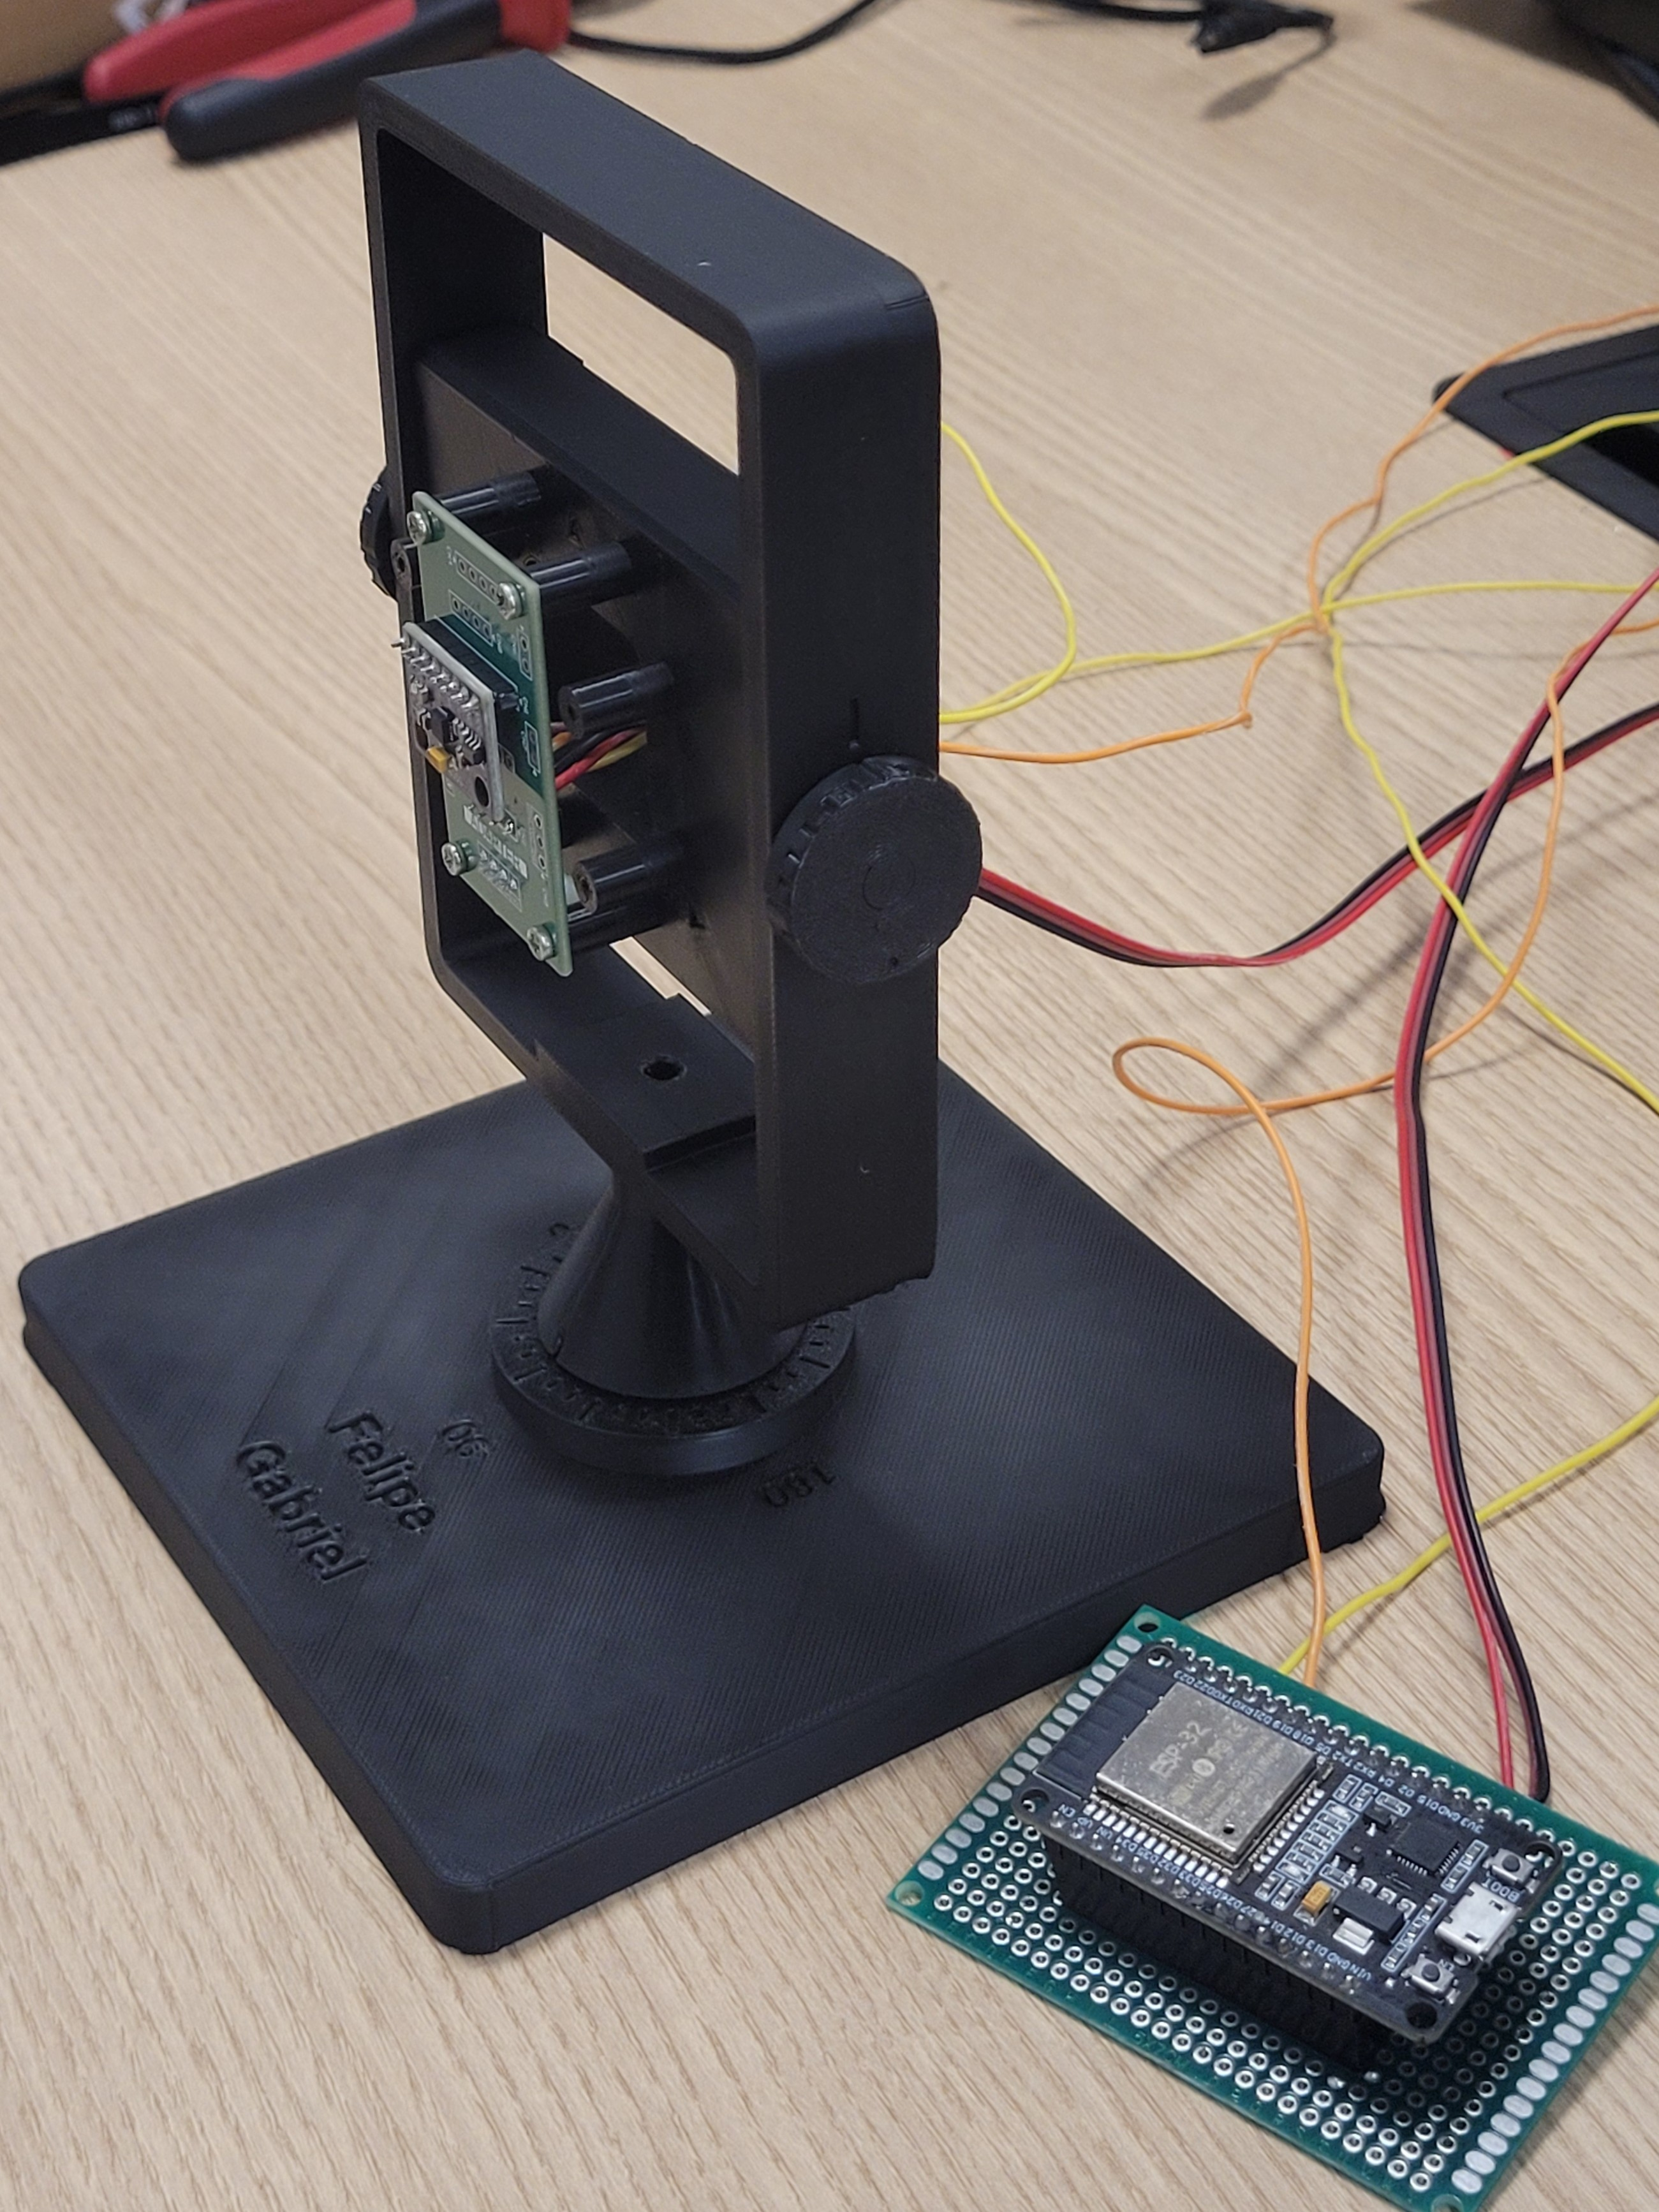
\includegraphics[width = 0.55\columnwidth]{Figuras/base__isometrico.jpg}}
	
	\vspace{0.3cm}
	
	\subfloat[Vista frontal.]{
		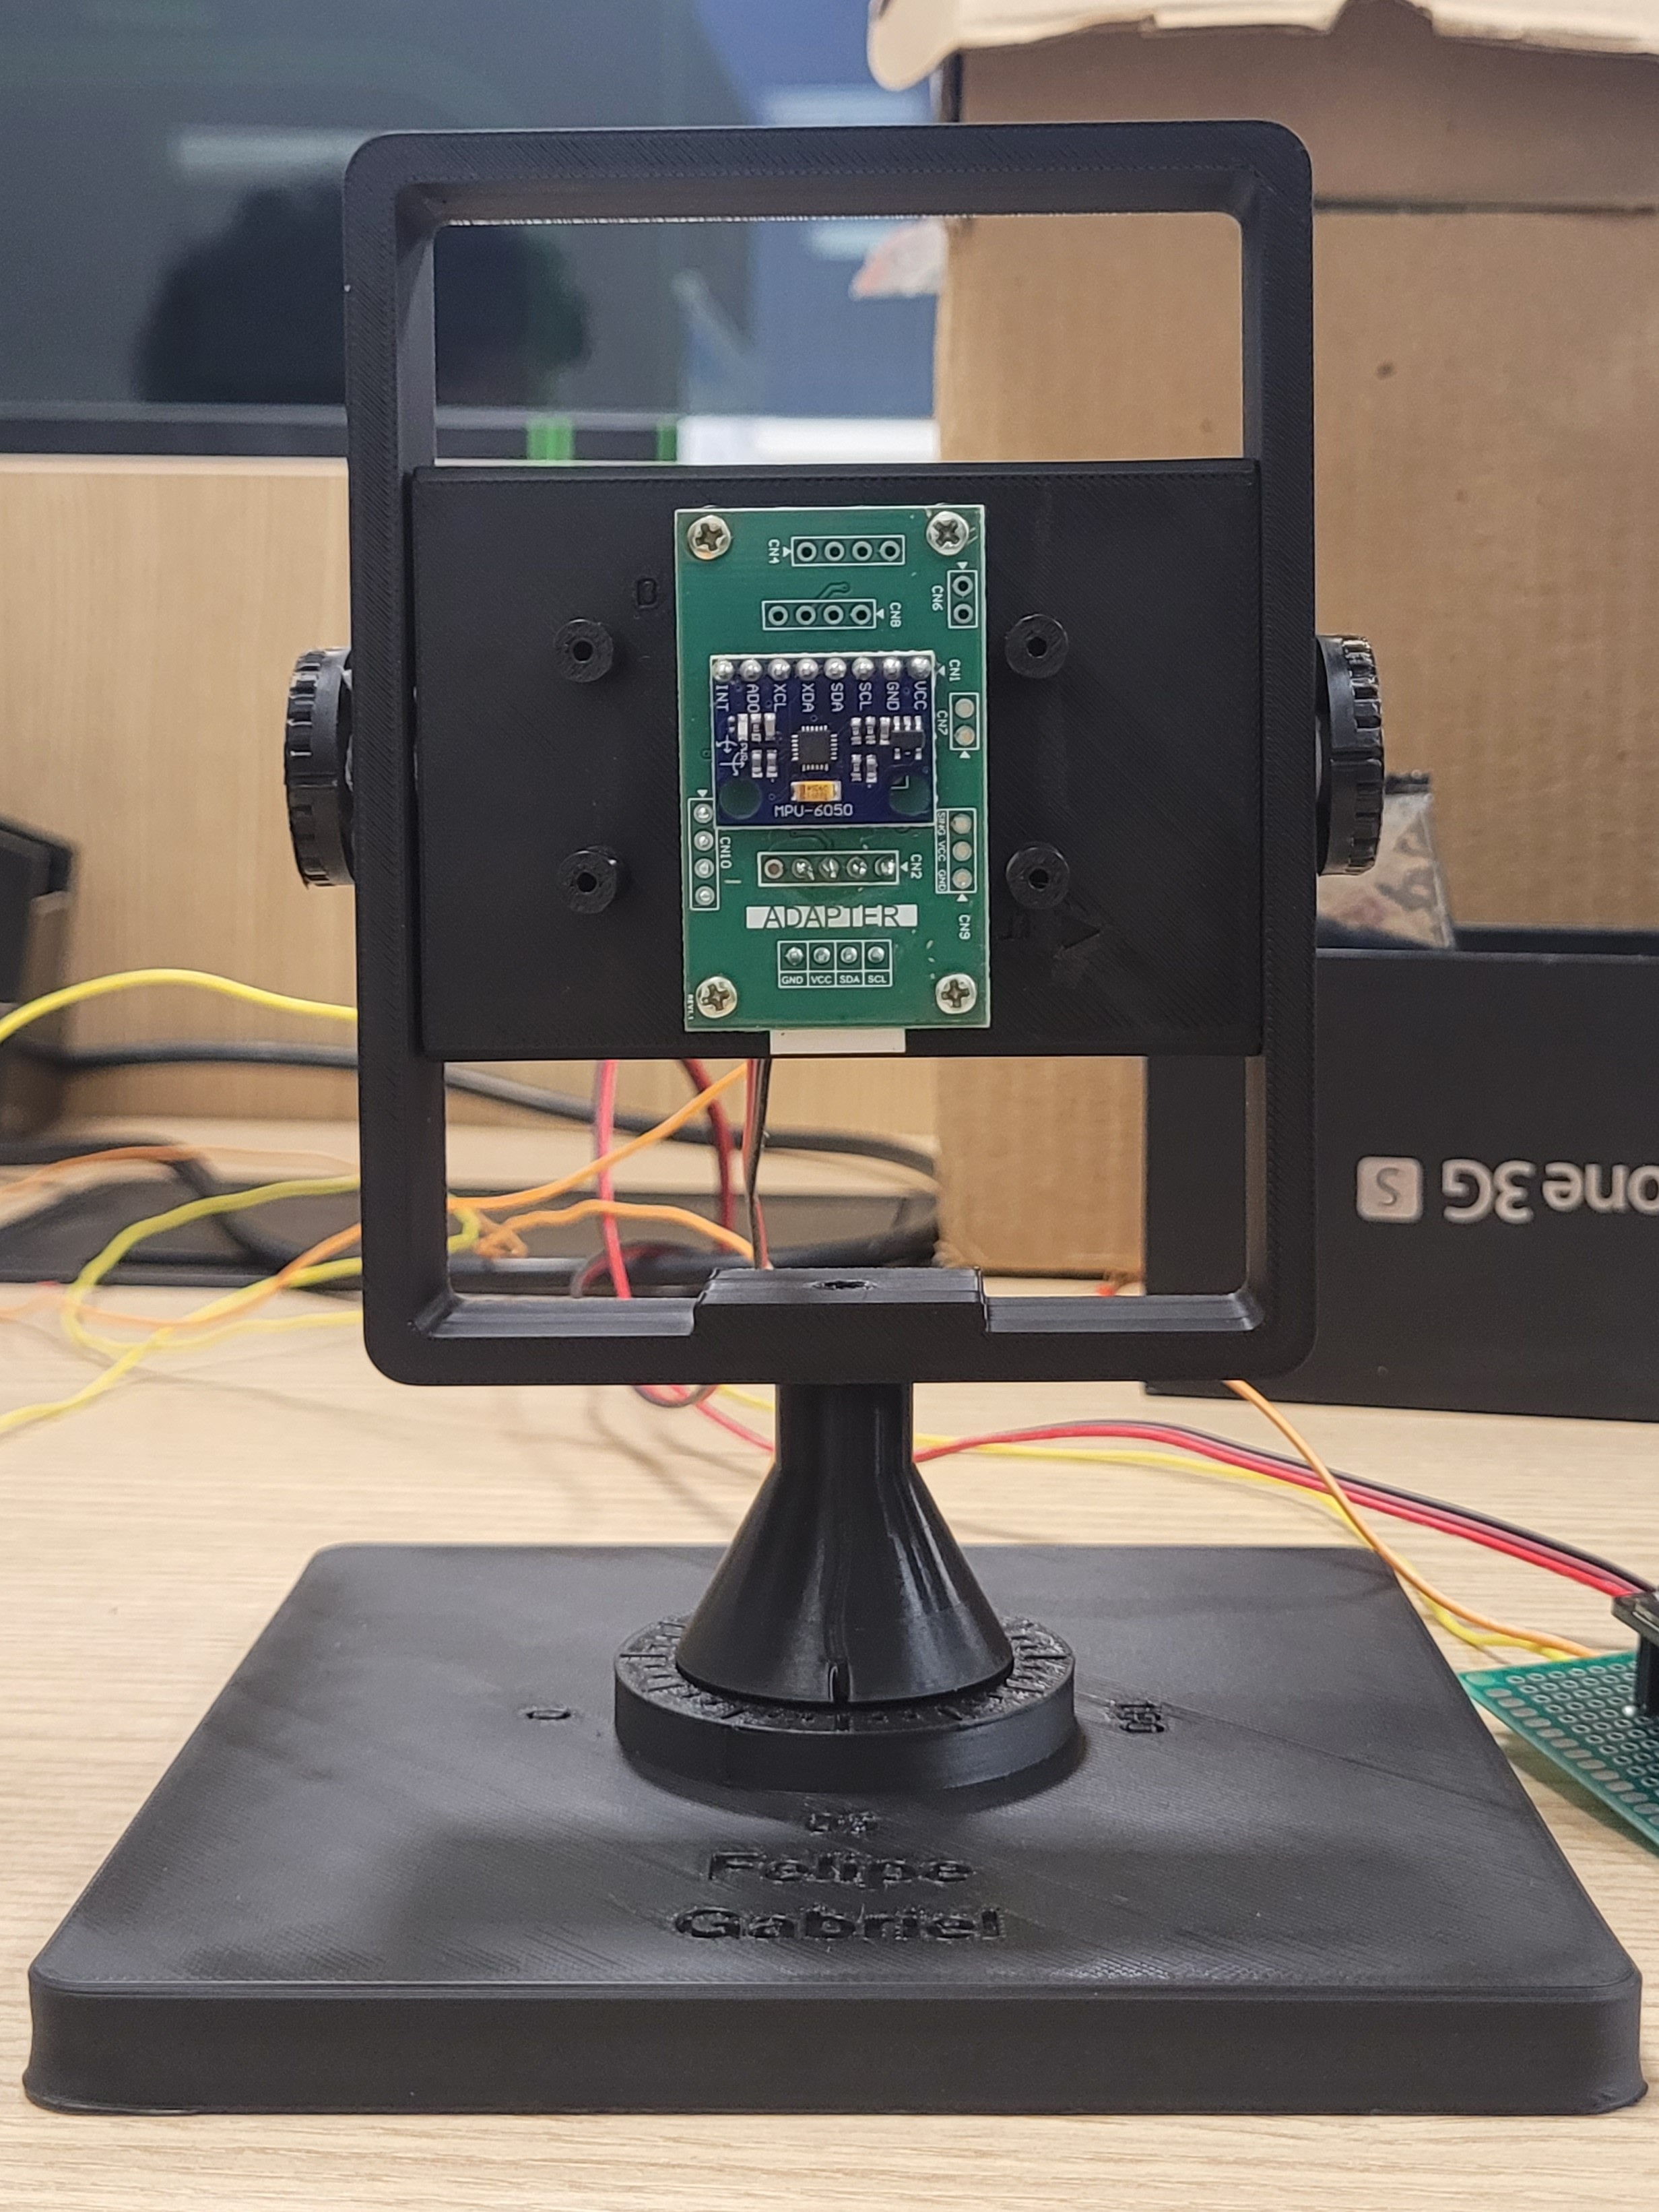
\includegraphics[width = 0.4\columnwidth]{Figuras/base_frontal.jpg}}
	\hfill
	\subfloat[Vista lateral.]{
		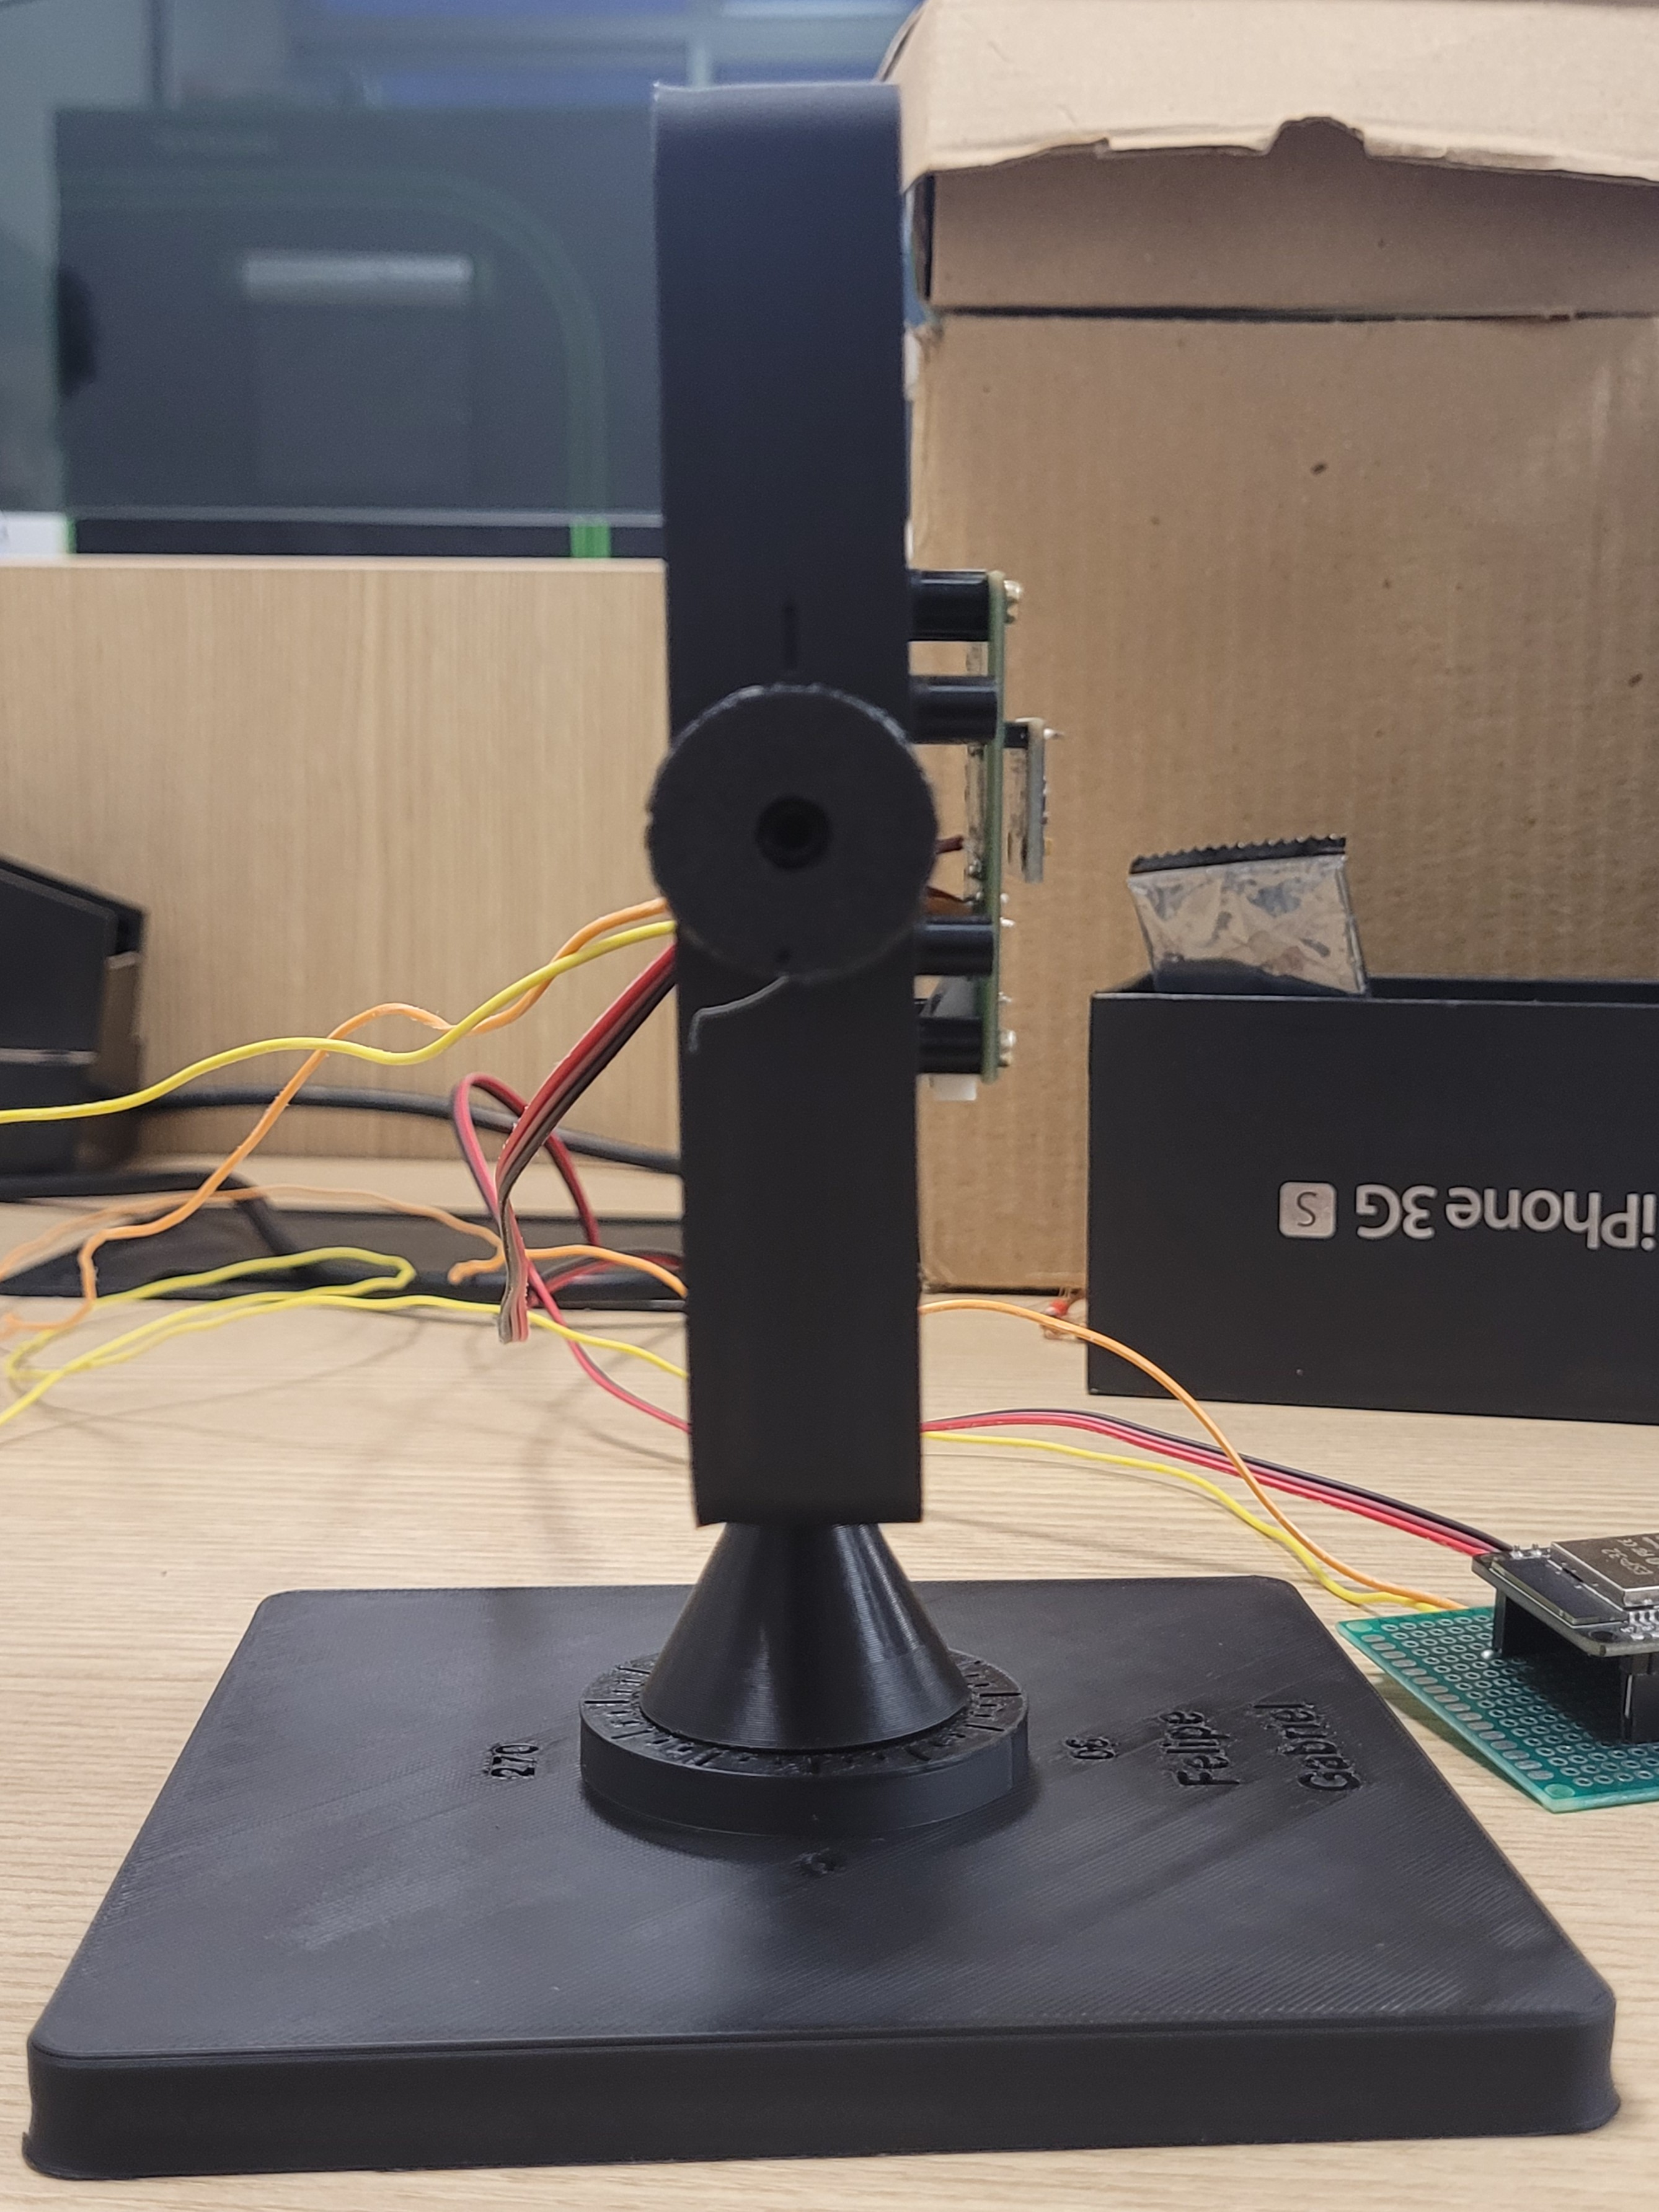
\includegraphics[width = 0.4\columnwidth]{Figuras/base_lateral.jpg}}
	\caption{Fotografia da base para calibração do MPU 6050 após montagem.}
	\label{fig:base_real}
\end{figure}

\subsection{Erro do Ângulo de Inclinação}
Com o firmware já calibrado, o braço foi colocado em 13 ângulos de referência, de $0^\circ$ a $180^\circ$ em passos de $15^\circ$. Em cada posição o berço foi travado e foram gravadas 100 leituras. O ângulo medido é a média dessas leituras, e o erro é a diferença entre o ângulo de referência e o ângulo medido. A Figura~\ref{fig:erro} mostra o erro ao longo da faixa.

Para comparar, a figura também mostra o erro sem calibração. Essa curva foi calculada com as leituras brutas de X, Y e Z que o firmware grava em cada linha junto com o ângulo corrigido, aplicando a Equação~\eqref{eq:atan2} sem a correção da Equação~\eqref{eq:correcao}. 

\begin{figure}[!t]
	\centering
	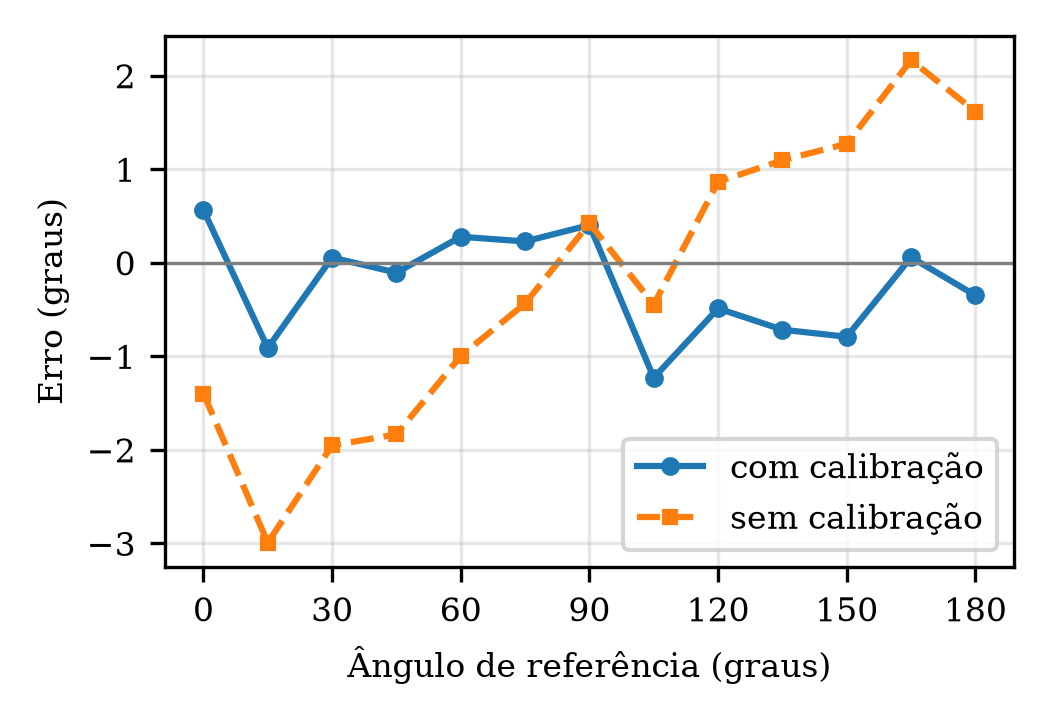
\includegraphics[width=\columnwidth]{Figuras/grafico_erro.png}
	\caption{Erro do ângulo (referência menos medido) em função do ângulo de referência. A curva com calibração é a saída do ESP32; a curva sem calibração foi calculada a partir das leituras brutas dos mesmos ensaios, sem a correção da Equação~\eqref{eq:correcao}.}
	\label{fig:erro}
\end{figure}

\section{Resultados}
% TODO: discussão dos resultados. Números dos dados (erro_angulo.py):
% - com calibração: erro médio -0,23 graus, maior erro -1,23 graus (em 105),
%   RMS 0,59 graus;
% - sem calibração: maior erro -2,99 graus (em 15); a curva sem calibração
%   cresce de cerca de -1,4 graus (em 0) até +1,6 graus (em 180), forma
%   esperada para o offset de 34 mg do eixo Z;
% - desvio-padrão das 100 leituras de cada ângulo: de 0,14 a 0,51 graus.

Ao calcularmos os erros médios entre os angulos medidos, raiz do erro quadrático médio (RMSE) e seus desvios padrões, exibidos na Tabela \ref{tab:erro_angulo}.

Percebe-se que após a a calibração tanto o erro máximo quanto o desvio padrão diminuiram, mostrando que a calibração do sensor torna seu comportamento mais exato. O erro médio se mantem similar pois os erros dos sensores possuem sinais diferentes e diminuem o valor do erro médio, por isso é importante considear o RMSE (Root Mean Square Error) e o desvio padrão para avaliar a precisão do sensor.

\begin{table}[h]
\centering
\caption{Erro do ângulo de inclinação com e sem calibração.}
\label{tab:erro_angulo}
\begin{tabular}{lcc}
\hline
Métrica & Com calibração & Sem calibração \\
\hline
Erro médio (${\degree}$)          & $-0{,}23$ & $-0{,}20$ \\
Maior erro (${\degree}$)          & $-1{,}23$ & $-2{,}99$ \\
Desvio padrão (${\degree}$)       & $0{,}56$ & $1{,}58$ \\
RMSE (${\degree}$)                & $0{,}65$ & $1{,}56$ \\
\hline
\end{tabular}
\end{table}

É importante considear que o transferidor utilizado para medir o ângulo de referência possui uma resolução de 1 grau, o que limita a precisão da medição do ângulo de referência. Além disso, é possivel que haja erros gerados pela inclinação do sensor no sentido diferente do que estava sendo medido, já que a base não possuia nivelamento perfeito.

\section{Conclusões}
% TODO: análise crítica dos objetivos e resultados, perspectivas e melhorias.

Neste trabalho, o acelerômetro do MPU 6050 foi caracterizado a partir da
folha de dados, verificado com o sensor em repouso, calibrado pelo método das
seis posições e usado para medir o ângulo de inclinação de um mecanismo de um
grau de liberdade, comparado a uma referência angular. A calibração resultou
em ganhos entre $0{,}9988$ e $1{,}0153$ e em um \textit{offset} de
$34{,}4$~mg no eixo Z, compatível com o valor típico de $\pm 80$~mg informado
no \textit{datasheet}.

Nos 13 ângulos ensaiados, de $0^\circ$ a $180^\circ$ em passos de $15^\circ$,
a calibração reduziu o RMSE de $1{,}56^\circ$ para $0{,}65^\circ$ (cerca de
58\%) e o maior erro médio de $2{,}99^\circ$ para $1{,}23^\circ$. O erro
médio praticamente não mudou ($-0{,}20^\circ$ e $-0{,}23^\circ$), porque os
erros sem calibração têm sinais alternados e se cancelam; por isso ele não
serve, sozinho, como medida de exatidão. 

Os resultados valem para as condições do ensaio: medição estática, uma única
unidade do sensor e com uma série de leituras por
ângulo. A referência angular, com resolução de $1^\circ$, também contribui
para o erro observado e limita a exatidão que pode ser afirmada. Como
melhorias, propõem-se calibrar o sensor já montado no mecanismo e com mais
orientações, usar uma referência angular mais exata.

\FloatBarrier % todas as figuras e tabelas saem antes das referências
\bibliographystyle{IEEEtran}
\bibliography{referencias}

\end{document}
